\chapter{Metodología y Diseño Experimental}
\label{capitulo:metodologia}

Este capítulo describe el diseño experimental, la operacionalización de las variables, la construcción de los escenarios de simulación y la arquitectura computacional utilizada. También presenta los protocolos de entrenamiento y evaluación empleados para comparar \acrshort{acr-mappo} y \acrshort{acr-happo} con las líneas de base \acrshort{acr-ippo} e \acrshort{acr-idqn}. El estudio adopta un enfoque cuantitativo y un diseño comparativo con replicaciones independientes y comparaciones pareadas por semilla: cada ejecución de entrenamiento produce una política y cada política se evalúa bajo semillas y condiciones de demanda previamente definidas. La simulación microscópica del tránsito funciona como un entorno controlado; el escenario de la Ciudad de Mendoza se interpreta como una construcción sintética restringida por datos parciales, no como un gemelo digital completo.

\section{Enfoque y Diseño de Investigación}
\label{sec:enfoque_diseno}

Este trabajo adopta un \textbf{diseño experimental cuantitativo comparativo con replicaciones independientes y comparaciones pareadas por semilla}. Los factores principales son la familia algorítmica, la arquitectura de la red neuronal, el grado de cooperación vecinal $\rho_{\mathrm{coop}}$ y el escenario de tránsito. Las políticas se comparan dentro de cada escenario y, de forma complementaria, se estudia cómo cambia su comportamiento al aumentar la escala o modificar la topología. Dado que también cambian la demanda y el número de agentes, las comparaciones entre escenarios se expresan mediante métricas absolutas y mediante variaciones relativas respecto del controlador de tiempo fijo del mismo escenario.

La simulación microscópica se utiliza como plataforma experimental por tres razones. El simulador utilizado es \acrshort{acr-sumo} \cite{SUMO2026_SUMO}:
\begin{enumerate}
    \item \textbf{Seguridad y viabilidad operacional:} evaluar algoritmos estocásticos de aprendizaje en tiempo real sobre una red urbana real implicaría riesgos para la seguridad vial y la fluidez del tránsito.
    \item \textbf{Aislamiento de variables exógenas:} la simulación permite controlar perturbaciones que no forman parte del modelo, como condiciones meteorológicas, siniestros viales o fluctuaciones externas.
    \item \textbf{Replicabilidad:} la fijación de semillas pseudoaleatorias permite someter los distintos controladores a las mismas condiciones de demanda.
\end{enumerate}

Para evaluar las políticas se emplean métricas físicas extraídas de la telemetría microscópica de \acrshort{acr-sumo}, principalmente del archivo \texttt{TripInfo}. La métrica primaria de la búsqueda de hiperparámetros es la espera media por vehículo insertado; las demás métricas se utilizan para interpretar eficiencia, atención de la demanda, equidad y estabilidad:
\begin{itemize}
    \item \textbf{Espera media de los vehículos insertados ($\bar{w}_{\mathrm{ins}}$):} métrica operacional obtenida de \texttt{TripInfo}:
    \begin{equation}
        \bar{w}_{\mathrm{ins}} = \frac{\sum_{v\in\mathcal{V}_{\mathrm{ins}}} w_v}{|\mathcal{V}_{\mathrm{ins}}|},
        \qquad w_v=\texttt{waitingTime}_v .
        \label{eq:espera_media_insertados}
    \end{equation}
    En la ecuación \eqref{eq:espera_media_insertados}, $\mathcal{V}_{\mathrm{ins}}$ es el conjunto de vehículos insertados en la ventana, $w_v$ es el tiempo de espera del vehículo $v$ en segundos y $|\mathcal{V}_{\mathrm{ins}}|$ es su cardinalidad. SUMO define \texttt{waitingTime} como el tiempo con velocidad menor o igual a $0,1\,\mathrm{m/s}$; por tanto, la métrica es un promedio en segundos por vehículo y no una suma en vehículo$\cdot$segundo. El entorno conserva además la espera integrada de los vehículos expuestos durante la ventana, pero esta magnitud no constituye el objetivo principal.
    \item \textbf{\gls{acr-cr}:} proporción de la demanda cargada que completa su itinerario dentro del horizonte de evaluación. La métrica también contabiliza los vehículos retenidos en los accesos de origen por sobresaturación:
    \begin{equation}
        \text{CR} = \frac{\text{throughput}}{\text{departed} + \text{pending\_vehicles\_end}}
        \label{eq:tasa_completitud}
    \end{equation}
    La ecuación \eqref{eq:tasa_completitud} relaciona los vehículos completados con la demanda que ingresó o quedó retenida. Todos sus términos son conteos del mismo horizonte: $\text{throughput}$ corresponde a los vehículos que completaron su itinerario, $\text{departed}$ a los que ingresaron a la calzada y $\text{pending\_vehicles\_end}$ a los que permanecieron en origen sin poder insertarse al cierre de la ventana. Cuando el simulador no descarta vehículos, se cumple la conservación $\text{loaded} \approx \text{departed} + \text{pending\_vehicles\_end}$ y el denominador de CR coincide con la carga de la ventana \cite{SUMO2026_SUMO}. También se registran la \gls{acr-ir} ($\text{IR} = \frac{\text{inserted}}{\text{loaded}}$) y la \gls{acr-ci} ($\text{CI} = \frac{\text{arrived\_inserted}}{\text{inserted}}$). Esta última tasa se restringe a los vehículos insertados durante la ventana que también completan su itinerario en ella; evita mezclar en el numerador vehículos presentes desde el calentamiento. Las tres tasas se informan conjuntamente con la métrica primaria porque un promedio calculado sobre los vehículos que circulan puede mejorar si un controlador restringe la inserción de demanda sin aliviar la congestión, efecto documentado en la evaluación de control semafórico por aprendizaje por refuerzo \cite{jiang2024xlight}.
    \item \textbf{Equidad espacial de demoras (coeficiente de Gini, $G_{\text{wait}}$):} cuantifica la desigualdad en la distribución del tiempo de espera medio entre las intersecciones semaforizadas de la red:
    \begin{equation}
        G_{\text{wait}} = \frac{2 \sum_{i=1}^{N} i \cdot \bar{w}_{(i)} - (N + 1) \sum_{i=1}^{N} \bar{w}_{(i)}}{N \sum_{i=1}^{N} \bar{w}_{(i)}}
        \label{eq:gini_espera}
    \end{equation}
    La ecuación \eqref{eq:gini_espera} se calcula después de ordenar los tiempos de espera medios. En ella, $\bar{w}_{(1)} \le \bar{w}_{(2)} \le \dots \le \bar{w}_{(N)}$ son los tiempos de espera medios ordenados de cada intersección y $N$ es el total de intersecciones semaforizadas. Cada $\bar{w}_i$ es el promedio temporal, sobre los pasos de decisión de la ventana controlada, de la espera media de los vehículos presentes en los carriles controlados por esa intersección. Las intersecciones entran con peso uniforme, sin ponderar por demanda: el índice describe la distribución interseccional del servicio, no la distribución entre vehículos individuales. Esta métrica se complementa con la desviación estándar inter-intersección ($\sigma_{\text{wait}}$) para evaluar si las políticas aprendidas distribuyen equitativamente el servicio o si sacrifican accesos secundarios en favor de arterias dominantes.
    \item \textbf{Pérdida temporal ($\overline{\ell}$):} promedio de \texttt{timeLoss} por vehículo insertado, que cuantifica el tiempo perdido respecto de la velocidad ideal del vehículo. Se registra como métrica secundaria porque incluye desaceleraciones y conflictos de circulación que no siempre se reflejan en la espera.
\end{itemize}

El archivo \texttt{TripInfo} solo incluye viajes finalizados cuando se escribe durante la ejecución; por eso el entorno activa \texttt{--tripinfo-output.write-unfinished} y cierra la conexión al terminar el episodio. Las métricas se calculan entonces sobre todos los registros válidos cuyo atributo de partida pertenece a la ventana, incluidos los viajes que aún no llegaron a destino. La documentación de SUMO define de forma independiente \texttt{waitingTime} y \texttt{timeLoss}; no se los intercambia en el análisis.

La figura \ref{fig:flujo_metodologico_general} resume las siete etapas de la investigación. En este contexto, \emph{etapa} designa una parte del procedimiento metodológico y no una fase del ciclo semafórico.

\begin{figure}[H]
\centering
\begin{tikzpicture}[
  node distance=0.35cm and 0cm,
  font=\sffamily\small,
  >=Stealth,
  paso/.style={rectangle, draw=colEntorno!80!black, fill=colEntorno!10, rounded corners=5pt, thick, text width=13.5cm, align=left, inner sep=6pt}
]
  \node[paso] (p1) {\textbf{1. Modelado Físico y Topológico de Redes:} Edición geométrica en \texttt{netedit}, auditoría topológica con Google Maps y Street View, reconstrucción de lógica semafórica y calibración de flota heterogénea.};
  \node[paso, below=of p1] (p2) {\textbf{2. Operacionalización del \acrshort{acr-decpomdp}:} especificación del vector de observaciones con codificación logarítmica (\texttt{Encoder}), espacio de acciones con enmascaramiento (\textit{action masking}) y recompensa local-vecinal $\rho_{\mathrm{coop}}$ (\texttt{neighborhood\_relevance}).};
  \node[paso, below=of p2] (p3) {\textbf{3. Desarrollo de la infraestructura del entorno:} abstracción en memoria compartida mediante \textit{bindings} en C++ (\texttt{libsumo}) e implementación de la interfaz \texttt{SumoRllibEnv} compatible con la \gls{acr-api} multiagente de Ray RLlib.};
  \node[paso, below=of p3] (p4) {\textbf{4. Configuración e integración algorítmica:} definición de arquitecturas neuronales en PyTorch (\gls{acr-mlp} $[128, 128]$ y $[256, 256]$) e hiperparámetros para \acrshort{acr-idqn}, \acrshort{acr-ippo}, \acrshort{acr-mappo} y \acrshort{acr-happo}.};
  \node[paso, below=of p4] (p5) {\textbf{5. Optimización de hiperparámetros (\acrshort{acr-hpo}):} muestreo bayesiano (Optuna \gls{acr-tpe}), poda asíncrona (\gls{acr-asha}) y función objetivo física de espera media con penalización de cola (\gls{acr-cvar}).};
  \node[paso, below=of p5] (p6) {\textbf{6. Orquestación y ejecución distribuida en \gls{acr-hpc}:} despliegue mediante \gls{acr-slurm} en los clústeres Toko y Mendieta, con almacenamiento local en nodo (\texttt{/scratch}) y aislamiento de puertos Ray.};
  \node[paso, below=of p6] (p7) {\textbf{7. Evaluación y confirmación:} comparación pareada en diez semillas, evaluación en semillas no utilizadas durante el ajuste, intervalos de confianza por bootstrap y análisis de eficiencia, completitud y equidad.};

  \draw[->, line width=1.2pt, colEntorno!80!black] (p1) -- (p2);
  \draw[->, line width=1.2pt, colEntorno!80!black] (p2) -- (p3);
  \draw[->, line width=1.2pt, colEntorno!80!black] (p3) -- (p4);
  \draw[->, line width=1.2pt, colEntorno!80!black] (p4) -- (p5);
  \draw[->, line width=1.2pt, colEntorno!80!black] (p5) -- (p6);
  \draw[->, line width=1.2pt, colEntorno!80!black] (p6) -- (p7);
\end{tikzpicture}
\caption{Flujo metodológico de la investigación experimental. Los siete recuadros representan, de arriba hacia abajo, las etapas de modelado de redes, formulación del problema, desarrollo del entorno, integración algorítmica, optimización de hiperparámetros, ejecución distribuida y evaluación estadística; las flechas indican la dependencia secuencial entre ellas.}
\label{fig:flujo_metodologico_general}
\end{figure}

La figura \ref{fig:flujo_metodologico_general} comienza con la construcción física y topológica de las redes que sirven como escenarios experimentales. Sobre esos escenarios se define el problema de decisión: qué observa cada agente, qué acciones puede ejecutar y qué recompensa recibe. La tercera etapa implementa esas definiciones en el entorno de simulación, y la cuarta incorpora los algoritmos y sus redes neuronales. Una vez que el sistema puede entrenarse, la quinta etapa busca configuraciones de hiperparámetros. La sexta distribuye las ejecuciones en la infraestructura de cómputo, y la séptima compara las políticas mediante métricas físicas y análisis de variabilidad. Las flechas verticales expresan la dependencia metodológica y no representan ejecución simultánea.

\section{Especificación del Ecosistema Tecnológico}
\label{sec:stack_tecnologico}

Para garantizar la reproducibilidad científica, la tabla \ref{tab:stack_tecnologico} detalla las librerías, marcos de trabajo y plataformas de cómputo sobre las cuales se desarrolló y ejecutó el entorno \texttt{marlTLC}. En esta sección, la \gls{telemetria} es el conjunto de mediciones que el simulador registra durante la ejecución; un \gls{framework} proporciona interfaces y componentes reutilizables para construir el sistema; un \gls{binding} conecta una biblioteca escrita en un lenguaje con otro, y la \gls{serializacion} convierte un objeto o mensaje en una representación que puede almacenarse o transmitirse. Los procesos denominados \textit{env runners} generan trayectorias al interactuar con el entorno y los \textit{learners} actualizan los parámetros de las redes a partir de esas trayectorias. Estas definiciones permiten interpretar la tabla sin suponer familiaridad previa con la infraestructura de software.

\begin{table}[H]
\centering
\caption{Especificación de las tecnologías y herramientas utilizadas en la investigación.}
\label{tab:stack_tecnologico}
\setlength{\tabcolsep}{5pt}
\small
\begin{tabular}{|>{\raggedright\arraybackslash}p{3.5cm}|>{\raggedright\arraybackslash}p{3.5cm}|>{\raggedright\arraybackslash}p{6.2cm}|}
\hline
\textbf{Componente} & \textbf{Herramienta / Versión} & \textbf{Función Metodológica} \\ \hline
Lenguaje de Programación & Python 3.10+ & Núcleo del sistema, tipado estático (\texttt{typing.Protocol}) y scripts de orquestación. \\ \hline
Simulador de Tránsito & \acrshort{acr-sumo} 1.20+ / \acrshort{acr-traci} & Simulación microscópica, dinámica cinemática y telemetría de red. \\ \hline
\textit{Bindings} de Simulación & \texttt{libsumo} (C++) & Ejecución de la simulación en memoria compartida mediante \textit{bindings} en C++ (\texttt{LIBSUMO\_AS\_TRACI=1}). \\ \hline
Marco de trabajo \acrshort{acr-marl} (\textit{framework}) & Ray RLlib 2.x \cite{liang2018rllib} & Abstracción de entornos multiagente (\texttt{MultiAgentEnv}, \texttt{RLModuleSpec}, \texttt{LearnerGroup}). \\ \hline
Aprendizaje Profundo & PyTorch 2.x & Modelado neuronal y optimización (Actor-Crítico \acrshort{acr-mlp}, \textit{action masking}). \\ \hline
Optimización Automática & Optuna 3.x \cite{akiba2019optuna} & Muestreo Bayesiano \acrshort{acr-tpe} y poda asíncrona de pruebas (\acrshort{acr-asha} \cite{li2020system}). \\ \hline
Infraestructura \acrshort{acr-hpc} & Clústeres Toko y Mendieta & Cómputo distribuido multinúcleo gestionado vía \acrshort{acr-slurm} con \gls{acr-es} local (\texttt{/scratch}). \\ \hline
\end{tabular}
\end{table}

Estas capas se integran de la siguiente manera. Python coordina la ejecución y Ray RLlib gestiona los procesos concurrentes de recolección de trayectorias (\textit{env runners}). PyTorch calcula las derivadas y optimiza las redes neuronales en los módulos de aprendizaje (\textit{learners}). \texttt{SumoRllibEnv} encapsula la lógica episódica y \texttt{libsumo} ejecuta los cálculos de cinemática vehicular en la memoria del proceso, sin comunicación por red ni serialización \gls{acr-tcp}.

\section[Diseño y Calibración de Escenarios de Tránsito en SUMO]{Diseño y Calibración de Escenarios de Tránsito en \acrshort{acr-sumo}}
\label{sec:diseno_escenarios}

La evaluación empírica se realiza sobre cuatro escenarios de red en \acrshort{acr-sumo}. Las redes se construyen con la herramienta gráfica \texttt{netedit}, los utilitarios de conversión \texttt{netconvert} y scripts de generación en Python. En conjunto, los escenarios representan distintas complejidades topológicas y condiciones de flujo.

\subsection{Modelado Geométrico y Sanitización Topológica}
\label{subsec:metodologia_modelado_sumo}

La construcción de las redes de simulación sigue un procedimiento de diseño y validación en \acrshort{acr-sumo}:
\begin{enumerate}
    \item \textbf{Diseño geométrico y accesos:} definición de calzadas, cantidad de carriles por aproximación y longitudes de almacenamiento en \texttt{netedit} o a partir de datos cartográficos de \acrshort{acr-osm}.
    \item \textbf{Auditoría y corrección topológica:} verificación de los sentidos de circulación, la cantidad de carriles, las conexiones de giro y las maniobras prohibidas. La revisión se contrasta con imágenes satelitales y vistas de calle de Google Maps y Google Street View.
    \item \textbf{Configuración semafórica:} las configuraciones de los semáforos estáticos corresponden a los planes generados por defecto por \acrshort{acr-sumo} (\texttt{netconvert --tls.rebuild}) al compilar la red. Los programas de fases y los tiempos de ciclo originales se mantienen sin cambios. La correspondencia entre los enlaces físicos y los índices de control semafórico (\textit{linkIndex}) se recalcula para conservar la consistencia topológica.
\end{enumerate}

\subsection{Escenarios Sintéticos: \texorpdfstring{$3\times1$, $3\times3$ y $4\times4\_H$}{3x1, 3x3 y 4x4-H}}
\label{subsec:escenarios_sinteticos}

Todas las redes sintéticas comparten las siguientes reglas operacionales:
\begin{itemize}
    \item \textbf{Límite de velocidad:} $13.89\text{ m/s}$ ($50\text{ km/h}$) en todas las arterias urbanas.
    \item \textbf{Flota vehicular heterogénea:} se definieron tres perfiles cinemáticos en el archivo \texttt{urban\_vehicle\_mix.add.xml}, a partir de los modelos disponibles en el simulador \cite{SUMO2026_SUMO}:
    \begin{enumerate}
        \item \texttt{SLOWVEHTYPE} ($25\%$): perfil de menor aceleración y velocidad máxima ($a = 1.9\text{ m/s}^2, d = 4.0\text{ m/s}^2, v_{\max} = 8.33\text{ m/s} = 30\text{ km/h}$).
        \item \texttt{MEDVEHTYPE} ($60\%$): perfil de referencia. Parámetros: $a = 2.6\text{ m/s}^2$ y $d = 4.5\text{ m/s}^2$; $v_{\max} = 13.89\text{ m/s} = 50\text{ km/h}$.
        \item \texttt{FASTVEHTYPE} ($15\%$): perfil de mayor aceleración, $a = 3.1\text{ m/s}^2$ y $d = 5.0\text{ m/s}^2$; $v_{\max} = 19.44\text{ m/s} = 70\text{ km/h}$.
    \end{enumerate}
    Parámetros compartidos: longitud $4.5\text{ m}$, brecha mínima de seguridad (\textit{minGap}) $2.5\text{ m}$ e imperfección del conductor de Krauss $\sigma = 0.5$.
    \item \textbf{Generación de demanda por zonas (\acrshort{acr-taz}):} las rutas se generan mediante \texttt{random\_routes\_taz.py} a partir de matrices de zonas de asignación de tránsito. Los tres escenarios sintéticos almacenan flujos con el atributo \texttt{vehsPerHour}; la demanda nominal se expresa en vehículos por hora y SUMO inserta los vehículos conforme al flujo solicitado. No se atribuye a estas redes un proceso de llegadas exponencial.
    \item \textbf{Calibración por bisección:} los flujos totales de los tres escenarios sintéticos se ajustaron mediante bisección bajo control semafórico de tiempo fijo, con el objetivo de obtener una tasa de completitud sobre los vehículos insertados (\acrshort{acr-ci}) próxima a $0,70$. El horizonte de referencia fue de $4200\text{ s}$, compuesto por $600\text{ s}$ de calentamiento y $3600\text{ s}$ de control.
\end{itemize}

La Tabla \ref{tab:escenarios_sinteticos} resume las características verificadas y los flujos nominales obtenidos para los tres escenarios sintéticos.

\begin{table}[H]
\centering
\caption{Características verificadas de los escenarios sintéticos.}
\label{tab:escenarios_sinteticos}
\small
\begin{tabular}{lrrrr}
\hline
\textbf{Escenario} & \textbf{Agentes} & \textbf{Tramos} & \textbf{Carriles} & \textbf{Flujo nominal (veh/h)} \\
\hline
$3\times1$ & 3 & 20 & 40 & 3.260 \\
$3\times3$ & 9 & 48 & 96 & 7.087 \\
$4\times4\_H$ & 16 & 71 & 166 & 7.202 \\
\hline
\end{tabular}
\end{table}

Los flujos finales de $3.260$ veh/h para $3\times1$, $7.087$ veh/h para $3\times3$ y $7.202$ veh/h para $4\times4_H$ fueron los obtenidos con esa calibración. El objetivo de completitud cercano a $0,70$ fija condiciones de congestión comparables para el estudio sintético; no establece una equivalencia exacta de demanda entre topologías ni valida una demanda urbana.

Las tres topologías sintéticas cumplen funciones analíticas complementarias:
\begin{itemize}
    \item \textbf{Corredor arterial $3\times1$ (3.260 veh/h):} tres intersecciones dispuestas en línea. El perfil canónico asigna explícitamente $40\%$ al par $3\to4$ y $35\%$ al par $4\to3$; el remanente se distribuye de forma reproducible entre los pares válidos restantes. Su disposición permite estudiar la propagación longitudinal de colas y la coordinación de fases sobre las corrientes predominantes.
    \item \textbf{Malla simétrica $3\times3$ (7.087 veh/h):} nueve intersecciones organizadas en una cuadrícula cerrada. El perfil canónico asigna $20\%$, $17,5\%$, $17,5\%$ y $20\%$ a los pares $5\to6$, $6\to5$, $10\to1$ y $1\to10$, respectivamente; el $25\%$ restante se asigna entre los pares válidos. La interconexión permite estudiar el desbordamiento de colas (\textit{spillback}) y la estabilidad de \acrshort{acr-marl} bajo congestión severa.
    \item \textbf{Cuadrícula $4\times4\_H$ (7.202 veh/h):} dieciséis intersecciones con geometría heterogénea. El perfil canónico asigna $20\%$, $17,5\%$, $17,5\%$ y $20\%$ a los pares $5\to9$, $6\to5$, $13\to1$ y $1\to13$, respectivamente; el $25\%$ restante se distribuye entre los pares válidos.
\end{itemize}

\subsection{Escenario urbano de la Ciudad de Mendoza}
\label{subsec:escenario_mendoza}

Para estudiar el comportamiento de los controladores en una red urbana de mayor escala, se construyó un escenario del microcentro de la Ciudad de Mendoza a partir de su infraestructura topológica y de una serie temporal parcial de aforo vehicular captada mediante una cámara termográfica. La red representa la geometría urbana, pero su demanda completa se aproxima mediante supuestos espaciales y un volumen nominal; por eso el escenario no se presenta como una validación del tránsito total de la ciudad. El diseño experimental prevé un ajuste de hiperparámetros, entrenamiento y evaluación propios para cada uno de los cuatro algoritmos en este escenario; no se transfieren pesos ni configuraciones finales desde las redes sintéticas.

\subsubsection{Posición Metodológica: Escenario Restringido por Datos}
\label{subsubsec:mendoza_posicion_metodologica}

El escenario de Mendoza se considera un \textbf{escenario sintético restringido por datos} (\textit{data-constrained synthetic scenario}), y no un gemelo digital completo.

La inferencia de una matriz \gls{acr-od} completa a partir de volúmenes medidos en pocos puntos de control es un problema inverso subdeterminado y mal condicionado \cite{calymayor, ite_handbook}. Para una red con $|\mathcal{Z}| = 37$ zonas de asignación de tránsito (\acrshort{acr-taz}), existen $|\mathcal{Z}|(|\mathcal{Z}|-1) = 1.332$ pares direccionales potenciales, de los cuales 520 son físicamente alcanzables. Este número contrasta con la cantidad limitada de enlaces instrumentados en el acceso oriental. Por lo tanto, las observaciones disponibles no determinan una única asignación \acrshort{acr-od}.

Por consiguiente, este trabajo utiliza dos criterios para construir la demanda:
\begin{enumerate}
    \item \textbf{Restricción dinámica empírica:} las mediciones continuas de aforo determinan el perfil horario de la demanda total y fijan el flujo observado en el corredor principal de ingreso.
    \item \textbf{Estructuración espacial híbrida:} la distribución espacial de los viajes combina un conocimiento previo (\textit{prior}) determinista, basado en la jerarquía vial, con un remanente estocástico controlado sobre los pares alcanzables.
\end{enumerate}

\subsubsection{Adquisición, Auditoría y Preprocesamiento de Telemetría Empírica}
\label{subsubsec:mendoza_preprocesamiento_datos}

La base empírica de aforo proviene de registros continuos de sensores de conteo y clasificación vehicular, correspondientes a cámaras térmicas Tecnotrans / \gls{acr-flir} ThermICam. Los registros tienen una resolución de 15 minutos y corresponden al período octubre de 2025 -- abril de 2026.

En las etapas preliminares se dispuso de información de cuatro dispositivos ubicados en el entorno del nudo de Costanera y Acceso Este. El relevamiento geoespacial mostró que las cámaras \texttt{192.168.1.167} (egreso hacia el este), \texttt{192.168.1.168} (circulación hacia el norte por Costanera) y \texttt{192.168.1.170} (circulación hacia el sur por Costanera) se encuentran entre $600\text{ m}$ y $800\text{ m}$ al este del perímetro de la red modelada. Por lo tanto, miden flujos de la autopista que quedan fuera del modelo vial urbano. En la generación y calibración definitiva se utiliza exclusivamente la Cámara 169 (\texttt{192.168.1.169}), ubicada en el viaducto sobre el canal Cacique Guaymallén, que registra el ingreso hacia el oeste por la Avenida José Vicente Zapata.

Para controlar la calidad de los datos de la Cámara 169, se aplicó un procedimiento de auditoría y saneamiento estructurado en cinco etapas:
\begin{enumerate}
    \item \textbf{Filtrado temporal y estructural:} descarte de marcas temporales corruptas, incluida la fecha anómala \texttt{1970-01-01}, o fuera del rango válido $[2020\text{--}2035]$.
    \item \textbf{Validación de zonas y clases vehiculares:} admisión de zonas válidas ($\text{ZoneID} \in [1, 19]$) y clasificación física en vehículos livianos ($l \le 5\text{ m}$), medianos ($5\text{ m} < l \le 10\text{ m}$) y pesados ($l > 10\text{ m}$), según $\text{ClassID} \in \{1, 2, 3\}$.
    \item \textbf{Eliminación de duplicados:} eliminación de registros redundantes mediante la clave $(\text{DateUTC}, \text{ZoneID}, \text{ClassID})$, conservando el último registro (\texttt{keep='last'}).
    \item \textbf{Alineación temporal:} reasignación de marcas con desviaciones $|\Delta t| \le 5\text{ s}$ al cuarto de hora más cercano y descarte de registros desalineados (\textit{off-grid}).
    \item \textbf{Filtro de días hábiles completos:} selección de días hábiles, de lunes a viernes, con cobertura del $100\%$ de los intervalos diarios de 15 minutos. El $95\%$ se utilizó como umbral operativo de auditoría antes de aplicar el criterio más estricto de inclusión.
\end{enumerate}

Este protocolo seleccionó $33$ días hábiles completos no perturbados, arrojando en la Cámara 169 un volumen empírico diario medio de $\mu_{\text{obs}} = 25.283,85\text{ veh/día}$ con una desviación estándar interdiaria de $\sigma_{\text{obs}} = 2.316,54\text{ veh/día}$.

\subsubsection{Mapeo Geoespacial, Corrección Topológica y Señalización}
\label{subsubsec:mendoza_topologia_red}

El trazado geométrico base se obtuvo mediante la exportación de datos de \acrshort{acr-osm} y su conversión al formato de red de \acrshort{acr-sumo} (\texttt{.net.xml}). El dominio modelado delimita el microcentro de la Ciudad de Mendoza entre Av. José Vicente Zapata / Colón al sur, Av. General San Martín como eje central norte-sur, Av. Manuel Belgrano al oeste y Av. Las Heras al norte. La red se proyecta en coordenadas \gls{acr-utm} Zona 19S (\gls{acr-wgs84}).

\paragraph{Punto de inyección este (\acrshort{acr-taz} 28):} dado que el nudo de Costanera se ubica al este del perímetro del modelo, la Cámara 169 se representa mediante el primer tramo interno disponible de la calzada de ingreso. Se utiliza el enlace (\textit{edge}) \texttt{93904440\#0}, asignado al origen de la zona \acrshort{acr-taz} 28.

\paragraph{Auditoría y corrección topológica con Google Maps y Street View:} tras la conversión inicial desde \acrshort{acr-osm}, se detectaron discrepancias entre la red y la infraestructura real. La red se revisó con imágenes satelitales de Google Maps y vistas de calle de Google Street View:
\begin{itemize}
    \item \textbf{Restricciones de giro y maniobras prohibidas:} se implementaron las restricciones observadas en terreno, como la prohibición de giro a la izquierda desde Av. General San Martín hacia el sur por Av. Colón. También se conservaron los giros semaforizados permitidos, como el de calle Perú hacia Av. Las Heras.
    \item \textbf{Sentidos de circulación y conectividad vial:} se corrigieron los sentidos de circulación de calzadas secundarias que figuraban como bidireccionales o invertidas en \acrshort{acr-osm}. También se restituyó la continuidad de los cuatro carriles de ingreso de la Av. José Vicente Zapata hacia la trama interior (\texttt{93904440\#0} a \texttt{93904440\#1}).
    \item \textbf{Cantidad de carriles y accesos laterales:} se ajustó el número de carriles de aproximación por calzada y se habilitaron las conexiones de inserción en las calles transversales Catamarca, Buenos Aires y Leandro N. Alem.
    \item \textbf{Configuración de semáforos estáticos y señalización:} las configuraciones de los semáforos de tiempo fijo corresponden a los programas generados por defecto por \acrshort{acr-sumo} (\texttt{--tls.rebuild}) al compilar la red. Las señalizaciones, las secuencias de fases y las duraciones de ciclo de la red modelada se mantuvieron sin cambios. Estos programas constituyen la línea base computacional del escenario; no se interpretan como una reconstrucción de los planes semafóricos municipales.
\end{itemize}

\subsubsection{Perfil temporal y factor de expansión territorial}
\label{subsubsec:mendoza_demanda_dinamica}

El flujo vehicular en cada paso temporal se modela a partir del perfil horario representativo $\bar{q}_{\text{obs}, 169}(h)$ ($h \in [0, 23]$), promediado sobre los 33 días hábiles completos. El análisis de distribución temporal revela que el período diurno de 12 horas ($06:00\text{--}18:00$) concentra el $69,29\%$ del flujo diario total, mientras que la ventana matutina de hora pico ($06:30\text{--}08:30$) concentra el $12,53\%$.

Para proyectar el aforo del enlace observado a la escala de la red, se aplica un \textbf{factor de expansión territorial constante} al perfil horario \cite{calymayor, ite_handbook}. El factor se basa en el volumen diario nominal $V_{\text{diario}} = 260.000\text{ veh/día}$, adoptado tras una exploración de sensibilidad en el rango $250.000\text{--}290.000\text{ veh/día}$:
    \begin{equation}
    f_{\text{exp}} = \frac{V_{\text{diario}}}{\sum_{h=0}^{23} \bar{q}_{\text{obs}, 169}(h)} = \frac{260.000}{25.283,85} \approx 10,2832
    \label{eq:factor_expansion_mendoza}
    \end{equation}
La ecuación \eqref{eq:factor_expansion_mendoza} compara el volumen diario objetivo con el volumen diario observado y, por ello, produce un factor adimensional. La demanda total de la red en la hora $h$ queda determinada por:
    \begin{equation}
    Q_{\text{red}}(h) = \bar{q}_{\text{obs}, 169}(h) \cdot f_{\text{exp}}
    \label{eq:demanda_red_horaria}
    \end{equation}
La ecuación \eqref{eq:demanda_red_horaria} conserva el perfil horario observado y lo escala al volumen nominal de la red mediante $f_{\text{exp}}$. Se adopta $\text{camera\_retention}=1,0$ como hipótesis de trabajo: la cámara mide un acceso parcial y no permite determinar qué fracción de cada viaje alcanza el dominio modelado. Por ello, este parámetro debe interpretarse como una decisión de construcción del escenario y no como una tasa de cobertura validada.

\subsubsection[Estructuración espacial de la demanda (60/40)]{Estructuración espacial de la demanda (60/40)}
\label{subsubsec:mendoza_contrato_od_v14}

A partir de las 37 zonas \acrshort{acr-taz}, se calcularon $520$ pares \acrshort{acr-od} físicamente alcanzables mediante \gls{acr-bfs} sobre el grafo de conectividad vial. La distribución de la demanda horaria $Q_{\text{red}}(h)$ se rige por el archivo \acrshort{acr-od} canónico utilizado en la campaña (versión interna v14), formulado como una partición híbrida:
    \begin{equation}
    p_{od} = \begin{cases}
    p_{od}^{\text{calib}} & \text{si } (o,d) \in \mathcal{P}_{\text{exp}} \quad \text{con} \quad \sum_{(o,d) \in \mathcal{P}_{\text{exp}}} p_{od}^{\text{calib}} = 0,60 \\
    0 & \text{si } (o,d) \in \mathcal{Z}_{\text{struct}} \\
    \frac{0,40}{|\mathcal{P}_{\text{libre}}|} \cdot \xi_{od} & \text{si } (o,d) \in \mathcal{P}_{\text{libre}} = \mathcal{P}_{\text{reach}} \setminus (\mathcal{P}_{\text{exp}} \cup \mathcal{Z}_{\text{struct}})
    \end{cases}
    \label{eq:contrato_od_v14}
    \end{equation}
    La ecuación \eqref{eq:contrato_od_v14} asigna a cada par origen-destino una única de las tres reglas de la partición. En ella, $\mathcal{P}_{\text{exp}}$ es el conjunto de pares explícitos, $\mathcal{Z}_{\text{struct}}$ los ceros estructurales, $\mathcal{P}_{\text{libre}}$ los pares libres alcanzables y $\xi_{od}\geq 0$ es un factor de asignación estocástica. Para que el remanente represente exactamente el $40\%$ de la demanda, estos factores se normalizan mediante $\sum_{(o,d)\in\mathcal{P}_{\text{libre}}}\xi_{od}=|\mathcal{P}_{\text{libre}}|$; si todos los pares reciben el mismo peso, entonces $\xi_{od}=1$. En consecuencia, la suma de las probabilidades de los pares explícitos positivos y del remanente libre es uno, mientras que los ceros estructurales no reciben demanda.

\paragraph{Componente fijo calibrado ($60\%$):} estructurado en $476$ entradas de \path{mendoza_od_proportions.json} (473 pares con cuotas positivas y 3 ceros directos), para incorporar hipótesis de jerarquía vial informadas por la inspección cartográfica y por el aforo disponible:
\begin{itemize}
    \item \textbf{Jerarquía de arterias principales:} priorización de los corredores Av. Vicente Zapata (\acrshort{acr-taz} 28), Av. General San Martín (\acrshort{acr-taz} 19/29), Av. Colón / Emilio Civit (\acrshort{acr-taz} 7), Av. Las Heras (\acrshort{acr-taz} 37/38) y Av. Manuel Belgrano (\acrshort{acr-taz} 0).
    \item \textbf{Intervención en \acrshort{acr-taz} 12 (Av. Perú):} reducción teórica del tráfico de origen en $-20\%$, con un desvío realizado de $-0,47\%$ respecto de la cuota objetivo de $0,03657$. La intervención buscó reducir la sobrecarga sobre calle San Lorenzo (\textit{edge} \texttt{249618899}), identificada durante la construcción del escenario como cuello de botella de distribución en la hora pico.
    \item \textbf{Incremento de recorridos pasantes en Patricias Mendocinas:} aumento de $+9,3\%$ en la cuota de pares longitudinales respecto de la línea base histórica, para representar la función de drenaje norte-sur de esta vía comercial.
\end{itemize}

\paragraph{Ceros estructurales ($\mathcal{Z}_{\text{struct}}$):} tres pares alcanzables, $0\to3$, $10\to5$ y $21\to17$, reciben una probabilidad de asignación $p_{od}=0,0$ en el archivo canónico. Así, el remanente aleatorio no asigna vehículos a esas maniobras, consideradas frágiles durante la construcción del escenario. Esta decisión reduce una fuente conocida de bloqueo en el escenario generado, pero no constituye una garantía general de ausencia de \textit{gridlock}.

\paragraph{Remanente estocástico ($40\%$) y selección de semilla:} el remanente se distribuye entre los pares libres mediante \texttt{random\_routes\_taz.py}. Durante el diseño del escenario se evaluaron 18 semillas pseudoaleatorias; 10 completaron la simulación continua de 12 horas sin teleports reportados. Se seleccionó la semilla \texttt{104773} por su cercanía a la cuota objetivo de la \acrshort{acr-taz} 12 entre las realizaciones estables, y se fijó la semilla de simulación de \acrshort{acr-sumo} en \texttt{104729} para la validación operativa de la red. La selección no buscó maximizar la completitud ni obtener una semilla estadísticamente representativa. Una vez validada, la especificación de demanda se congeló en \texttt{mendoza\_12h.rou.xml}: el archivo fija los pares origen-destino, las tasas horarias y la mezcla de flota, mientras que los instantes de inserción se sortean durante la simulación conforme al proceso exponencial descrito más abajo. Las comparaciones algorítmicas usan esa misma especificación de demanda y, dentro de cada réplica pareada, la misma semilla de \acrshort{acr-sumo} para todos los controladores. Las semillas reservadas producen realizaciones adicionales de llegadas y dinámica; por ello, cuantifican la variabilidad de la simulación bajo el escenario definido y no la incertidumbre de la demanda urbana real.

\paragraph{Dinámica microscópica y heterogeneidad de flota:} las inserciones se programan como procesos de Poisson. Para cada par origen-destino, si $Q_{od}$ es el flujo en vehículos por hora, la tasa de arribos es $\lambda_{od} = \frac{Q_{od}}{3600}\text{ veh/s}$ y cada intervalo se obtiene como $H_{od} = -\ln(U)/\lambda_{od}$, con $U \sim \mathcal{U}(0,1)$. Así, el intervalo tiene unidad de segundos y valor esperado $\mathbb{E}[H_{od}] = 1/\lambda_{od} = 3600/Q_{od}\text{ s}$. En el archivo de rutas, \texttt{period="exp(rate)"} designa este muestreo exponencial; no significa calcular $e^{\lambda_{od}}$. La distribución de flota urbana heterogénea \texttt{td\_urban\_mix} está compuesta por 25\% de vehículos lentos, 60\% estándar y 15\% dinámicos.

\subsubsection{Protocolo de Validación Operacional y Criterio \acrshort{acr-geh}}
\label{subsubsec:mendoza_validacion_operacional}

La validación operacional se definió sobre dos horizontes temporales:
\begin{enumerate}
    \item \textbf{Escenario base canónico (12 horas, $06:00\text{--}18:00$):} horizonte experimental completo de $43.200\text{ s}$, que reproduce la evolución continua del tránsito diurno.
    \item \textbf{Ventana operacional (2 horas, $06:30\text{--}08:30$):} recorte temporal de la hora pico ($t = [1800, 9000]\text{ s}$), utilizado para la exploración iterativa de controladores y las evaluaciones de alta demanda.
\end{enumerate}

En ambos horizontes se registran los vehículos cargados, insertados y completados, junto con \acrshort{acr-cr}, inserción, completitud y activaciones del mecanismo \textit{teleport}. Estas mediciones permiten verificar que el escenario se mantiene operable antes de evaluar controladores; sus valores se presentan en el capítulo \ref{capitulo:resultados}.

\paragraph{Validación de calidad del flujo (estadístico \acrshort{acr-geh}):} conforme a las recomendaciones para la calibración de demanda en simulación microscópica \cite{SUMO2026_SUMO, ite_handbook}, la consistencia de la inyección en el corredor José Vicente Zapata (\acrshort{acr-taz} 28) respecto de los aforos de la Cámara 169 se evalúa mediante el estadístico \acrshort{acr-geh}:
\begin{equation}
    \text{GEH} = \sqrt{\frac{2 (V_{\mathrm{mod}} - V_{\mathrm{obs}})^2}{V_{\mathrm{mod}} + V_{\mathrm{obs}}}}
    \label{eq:geh}
\end{equation}
donde $V_{\mathrm{mod}}$ es el volumen horario modelado y $V_{\mathrm{obs}}$ el conteo horario empírico observado, ambos expresados en vehículos por hora. La ecuación \eqref{eq:geh} resume la discrepancia entre ambos volúmenes en una magnitud adimensional. En este trabajo, el estadístico se interpreta como una comprobación de consistencia entre el flujo solicitado en el acceso representado por la cámara y el aforo observado, no como evidencia de que la matriz \acrshort{acr-od} completa sea verdadera: los flujos del corredor se construyeron a partir de ese mismo aforo, por lo que la comparación verifica la implementación del perfil horario, no la demanda total. Al informar este cálculo se declaran el archivo de rutas, la ventana temporal y la hipótesis de retención; las versiones anteriores del escenario se documentan como antecedentes de construcción y no se combinan con la evaluación del escenario canónico.

\section{Arquitectura de Integración Entorno-Agentes}
\label{sec:arquitectura_entorno_agentes}

El marco computacional \texttt{marlTLC} integra el simulador \acrshort{acr-sumo} con la librería Ray RLlib a través de la interfaz personalizada \texttt{SumoRllibEnv}. La especificación detallada de las clases y patrones de diseño orientados a objetos que sustentan esta arquitectura se expone en el Apéndice \ref{apendice:arquitectura_software}.

\subsection{Ciclo Episódico e Interfaz de Simulación}
\label{subsec:ciclo_episodico}

Para mejorar la recolección de muestras durante el entrenamiento distribuido, las simulaciones se ejecutan sin interfaz gráfica. En los trabajos por lote se activa la variable de entorno \path{LIBSUMO_AS_TRACI=1}, con lo que Python utiliza el \textit{binding} nativo \texttt{libsumo}; cuando la variable no está presente, el mismo código puede utilizar una conexión TraCI estándar. La primera opción evita la comunicación por sockets entre procesos del simulador y el entorno, mientras que ambas exponen la misma interfaz de control.

La conexión se configura en \texttt{sumo\_env.py} con un único objeto activo por entorno. Las opciones comunes fijan \texttt{--waiting-time-memory}, \texttt{--end} y la semilla de SUMO; cuando se solicita telemetría, se añade \texttt{--tripinfo-output} junto con \path{--tripinfo-output.write-unfinished}. En las ejecuciones por lote se desactivan \texttt{--no-}\allowbreak\texttt{step-log} y \texttt{--no-}\allowbreak\texttt{warnings} para reducir E/S innecesaria. La conexión TraCI convencional se inicia con una etiqueta propia y hasta diez reintentos, mientras que \texttt{libsumo} reutiliza la misma interfaz sin abrir un puerto. Al reiniciar un episodio, el entorno elimina el archivo de telemetría anterior, carga el estado de calentamiento con \texttt{simulation.loadState} y limpia los contadores de vehículos, teletransportes, espera y equidad; así se evita repetir el calentamiento y se impide que una ejecución contamine a la siguiente. El mapa de vecinos se construye una sola vez a partir de los carriles controlados y sus enlaces, con un recorrido de complejidad $O(TLC)$ en lugar de comparar todos los pares de semáforos, donde $T$ es el número de agentes, $L$ el número de carriles controlados y $C$ el número de conexiones inspeccionadas.

El ciclo de vida episódico opera bajo el siguiente protocolo de inicialización y control:
\begin{enumerate}
    \item \textbf{Período de calentamiento (\textit{warmup}):} los escenarios sintéticos utilizan $600\,\mathrm{s}$ bajo control semafórico de tiempo fijo. En la configuración MARL de Mendoza para dos horas, el archivo \texttt{.sumocfg} comienza en $t=1500\text{ s}$ (06:25), el calentamiento dura $300\,\mathrm{s}$ y la ventana controlada queda así en $[1800, 9000]\text{ s}$ (06:30--08:30), coincidente con el recorte de la hora pico. Esta fase puebla la red y evita que los agentes aprendan únicamente sobre una red vacía.
    \item \textbf{Almacenamiento y restauración de puntos de control (\textit{checkpoint}):} al finalizar el calentamiento, el estado microscópico de la red se almacena en un archivo \acrshort{acr-xml} (\texttt{state\_pid...xml}). Cada invocación de \texttt{reset()} restaura este estado, de modo que el entrenamiento comienza en condiciones equivalentes sin repetir la simulación preliminar. El tiempo controlado se interpreta como un intervalo absoluto cuando el archivo \texttt{.sumocfg} tiene un valor de inicio distinto de cero.
    \item \textbf{Paso de decisión y transiciones semafóricas:} las decisiones se ejecutan en pasos de $\Delta t = 5.0\text{ s}$. Cuando un agente cambia la fase activa, el entorno intercala una fase amarilla de $\text{yellow\_time} = 4\text{ s}$ y exige un tiempo mínimo de verde de $\text{min\_green\_time} = 5\text{ s}$ antes de habilitar la nueva transición.
\end{enumerate}

\section[Instanciación del modelo Dec-POMDP]{Instanciación del Modelo \acrshort{acr-decpomdp}}
\label{sec:instanciacion_dec_pomdp}

La interacción distribuida entre las intersecciones semaforizadas se formaliza como un juego parcialmente observable con observaciones locales. La notación de \acrshort{acr-decpomdp} del marco teórico se utiliza para describir la información disponible y la acción conjunta. En la implementación, cada controlador recibe una recompensa individual compuesta; la coordinación se induce mediante el componente vecinal de esa señal y el crítico centralizado durante el entrenamiento de MAPPO y HAPPO, no mediante la suma de todas las recompensas en un escalar global. La formulación difiere así del Dec-POMDP cooperativo canónico en la señal de retorno: el objetivo que optimiza cada actor es su retorno individual local-vecinal. Las comparaciones entre familias algorítmicas miden, en consecuencia, el desempeño de procedimientos completos de aprendizaje y coordinación, y no aíslan causalmente cada componente.

\subsection{Observaciones y codificación logarítmico-lineal}
\label{subsec:observaciones_encoder}

La observación local $o_i^{(t)}$ recibida por el agente $i$ en el paso $t$ combina el índice de la fase activa y una representación por carril de la espera acumulada:
\begin{equation}
 o_i^{(t)}=\bigl(p_i^{(t)},e(w_{i,1}^{(t)}),\ldots,e(w_{i,m_i}^{(t)})\bigr),
 \label{eq:observacion_local_metodologia}
\end{equation}
donde $p_i^{(t)}$ es el índice de la fase, $m_i$ es el número de carriles de entrada controlados por la intersección y $w_{i,l}^{(t)}$ es la espera acumulada atribuida al carril $l$ en el paso $t$: la suma de los tiempos de espera acumulados de los vehículos presentes en ese carril, expresada en vehículo$\cdot$segundo. La atribución recorre los vehículos y asigna a cada carril la contribución no registrada en los carriles anteriores, de modo que un vehículo que cambia de carril no duplica automáticamente su espera. En la configuración de las campañas de ajuste, la observación vecinal no se concatena al actor mediante \texttt{neighbor\_info=False}; la información de los vecinos se utiliza en la señal de recompensa y en la observación conjunta del crítico centralizado.

Para representar esta información se aplica la clase \texttt{Encoder} de \path{src/marlTLC/utils/encoder.py}. La transformación cuantiza cada espera en uno de $I$ niveles y conserva más resolución en el rango bajo. Así, valores de espera próximos que caen en el mismo intervalo quedan representados por una misma categoría, mientras que la saturación agrupa los valores iguales o superiores a $M_{\mathrm{lane}}$. Esta reducción de la variedad de valores codificados puede ofrecer una representación más manejable para el aprendizaje; el nivel de detalle adicional en esperas bajas busca retener distinciones relevantes en ese rango. Son motivaciones de diseño, no efectos de aprendizaje o rendimiento demostrados por separado: el redondeo puede perder distinciones relevantes y generar cambios de categoría al cruzar un umbral. La evaluación estudia el codificador integrado al sistema y no incluye una ablación frente a otras representaciones. Analíticamente, la función se construye como una combinación convexa en el dominio normalizado adimensional. Sea $x \ge 0$ la espera acumulada del carril y $M_{\mathrm{lane}} > 0$ su cota de saturación, ambas expresadas en la misma unidad física (vehículo$\cdot$segundo). Se define la variable adimensional normalizada $\hat{x} = \min(1, x / M_{\mathrm{lane}}) \in [0, 1]$. En dicho dominio unitario, se combinan un mapeo logarítmico cóncavo y un mapeo lineal mediante una mezcla convexa $g(\hat{x}) \in [0, 1]$:
\begin{equation}
    g(\hat{x}) = (1 - L) \frac{\log_2\left(\frac{\hat{x}}{L} + 1\right)}{\log_2\left(\frac{1}{L} + 1\right)} + L \hat{x},
    \label{eq:encoder_mezcla_convexa}
\end{equation}
donde $I \ge 2$ es el número de intervalos discretos y $L = (I - 1)/M_{\mathrm{lane}}$ actúa como parámetro numérico de curvatura y ponderación lineal. Con los rangos de $I$ y $M_{\mathrm{lane}}$ empleados en las configuraciones, $0<L<1$, por lo que los pesos de la combinación son positivos. Dado que $g(0) = 0$ y $g(1) = 1$, la curva mapea continuamente $[0, 1]$ sobre sí mismo. Para cuantizar la señal en el conjunto discreto $\{0, \dots, I - 1\}$, la salida se escala por el índice máximo $(I - 1)$ y se aplica la función techo ($\operatorname{ceil}$): $e(x) = \min\{I - 1, \operatorname{ceil}((I - 1) g(\hat{x}))\}$.

Al expandir algebraicamente $(I - 1) g(\hat{x})$ mediante las relaciones $(I - 1) = L \cdot M_{\mathrm{lane}}$, $\hat{x} / L = x / (M_{\mathrm{lane}} L)$ y $(I - 1) L \hat{x} = L^2 x$, se obtiene de forma exacta la expresión evaluada computacionalmente en el código:
\begin{equation}
    e(x) = \operatorname{ceil}\left( F \cdot \log_2\left( \frac{x}{M_{\mathrm{lane}} \cdot L} + 1 \right) + L^2 \cdot x \right),
    \label{eq:encoder_log_lineal}
\end{equation}
con $F = (1 - L)(I - 1) / \log_2(1/L + 1)$. Para $0 \le x < M_{\mathrm{lane}}$, la ecuación \eqref{eq:encoder_log_lineal} es la factorización compacta de la combinación convexa continua escalada por $(I - 1)$; para $x \ge M_{\mathrm{lane}}$, la implementación satura directamente la salida en $I - 1$. La función $\operatorname{ceil}$ redondea hacia arriba al entero más cercano. La letra $M_{\mathrm{lane}}$ se utiliza aquí exclusivamente para el codificador y no debe confundirse con el factor de ventaja $M$ de HAPPO.

En esta formulación:
\begin{itemize}
    \item \textbf{Número de intervalos ($I$):} corresponde al hiperparámetro \texttt{encoder\_intervals}, explorado en el rango entero $[4,64]$. La clase almacena internamente $I-1$ como el índice máximo, por lo que la salida pertenece a $\{0,\ldots,I-1\}$.
    \item \textbf{Cota de saturación del carril ($M_{\mathrm{lane}}$):} corresponde a \texttt{max\_lane\_value}, determinado empíricamente calculando el percentil 99 ($P_{99}$) de las esperas acumuladas por carril en simulaciones preliminares de cada red: $M_{\mathrm{lane}} = 1184$ vehículo$\cdot$segundo para $3\times1$, $M_{\mathrm{lane}} = 1136$ vehículo$\cdot$segundo para $3\times3$, $M_{\mathrm{lane}} = 712$ vehículo$\cdot$segundo para $4\times4\_H$ y $M_{\mathrm{lane}} = 1494$ vehículo$\cdot$segundo para el microcentro de la Ciudad de Mendoza.
\end{itemize}

La variable \texttt{lane\_metric} determina qué cantidad se extrae antes de codificar: la configuración utilizada en el ajuste es \texttt{acc\_waiting\_time}, definida arriba, mientras que el entorno también admite la espera del último paso y la cantidad de vehículos detenidos.

La observación ubica primero el índice de fase y luego los valores codificados de los carriles, en el orden definido por el entorno. La figura \ref{fig:codificacion_carriles} muestra la discretización escalonada de una espera, mientras que la figura \ref{fig:mezcla_log_lineal} ilustra la mezcla logarítmica-lineal. Estas figuras son auxiliares: la definición reproducible de la observación es la ecuación \eqref{eq:observacion_local_metodologia}, y la función de codificación se implementa en \texttt{src/marlTLC/utils/encoder.py}.

\begin{figure}[H]
    \centering
    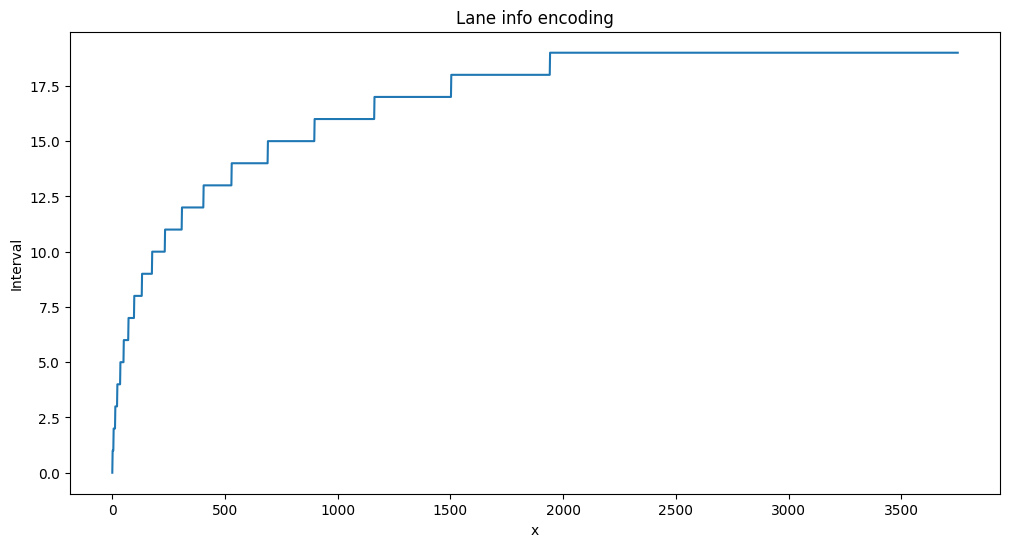
\includegraphics[width=0.78\textwidth]{imagenes/LaneInfoEncoding.png}
    \caption{Codificación por carril empleada para construir la observación local. Cada entrada de espera se transforma y conserva su correspondencia espacial con el carril de origen.}
    \label{fig:codificacion_carriles}
\end{figure}

\begin{figure}[H]
    \centering
    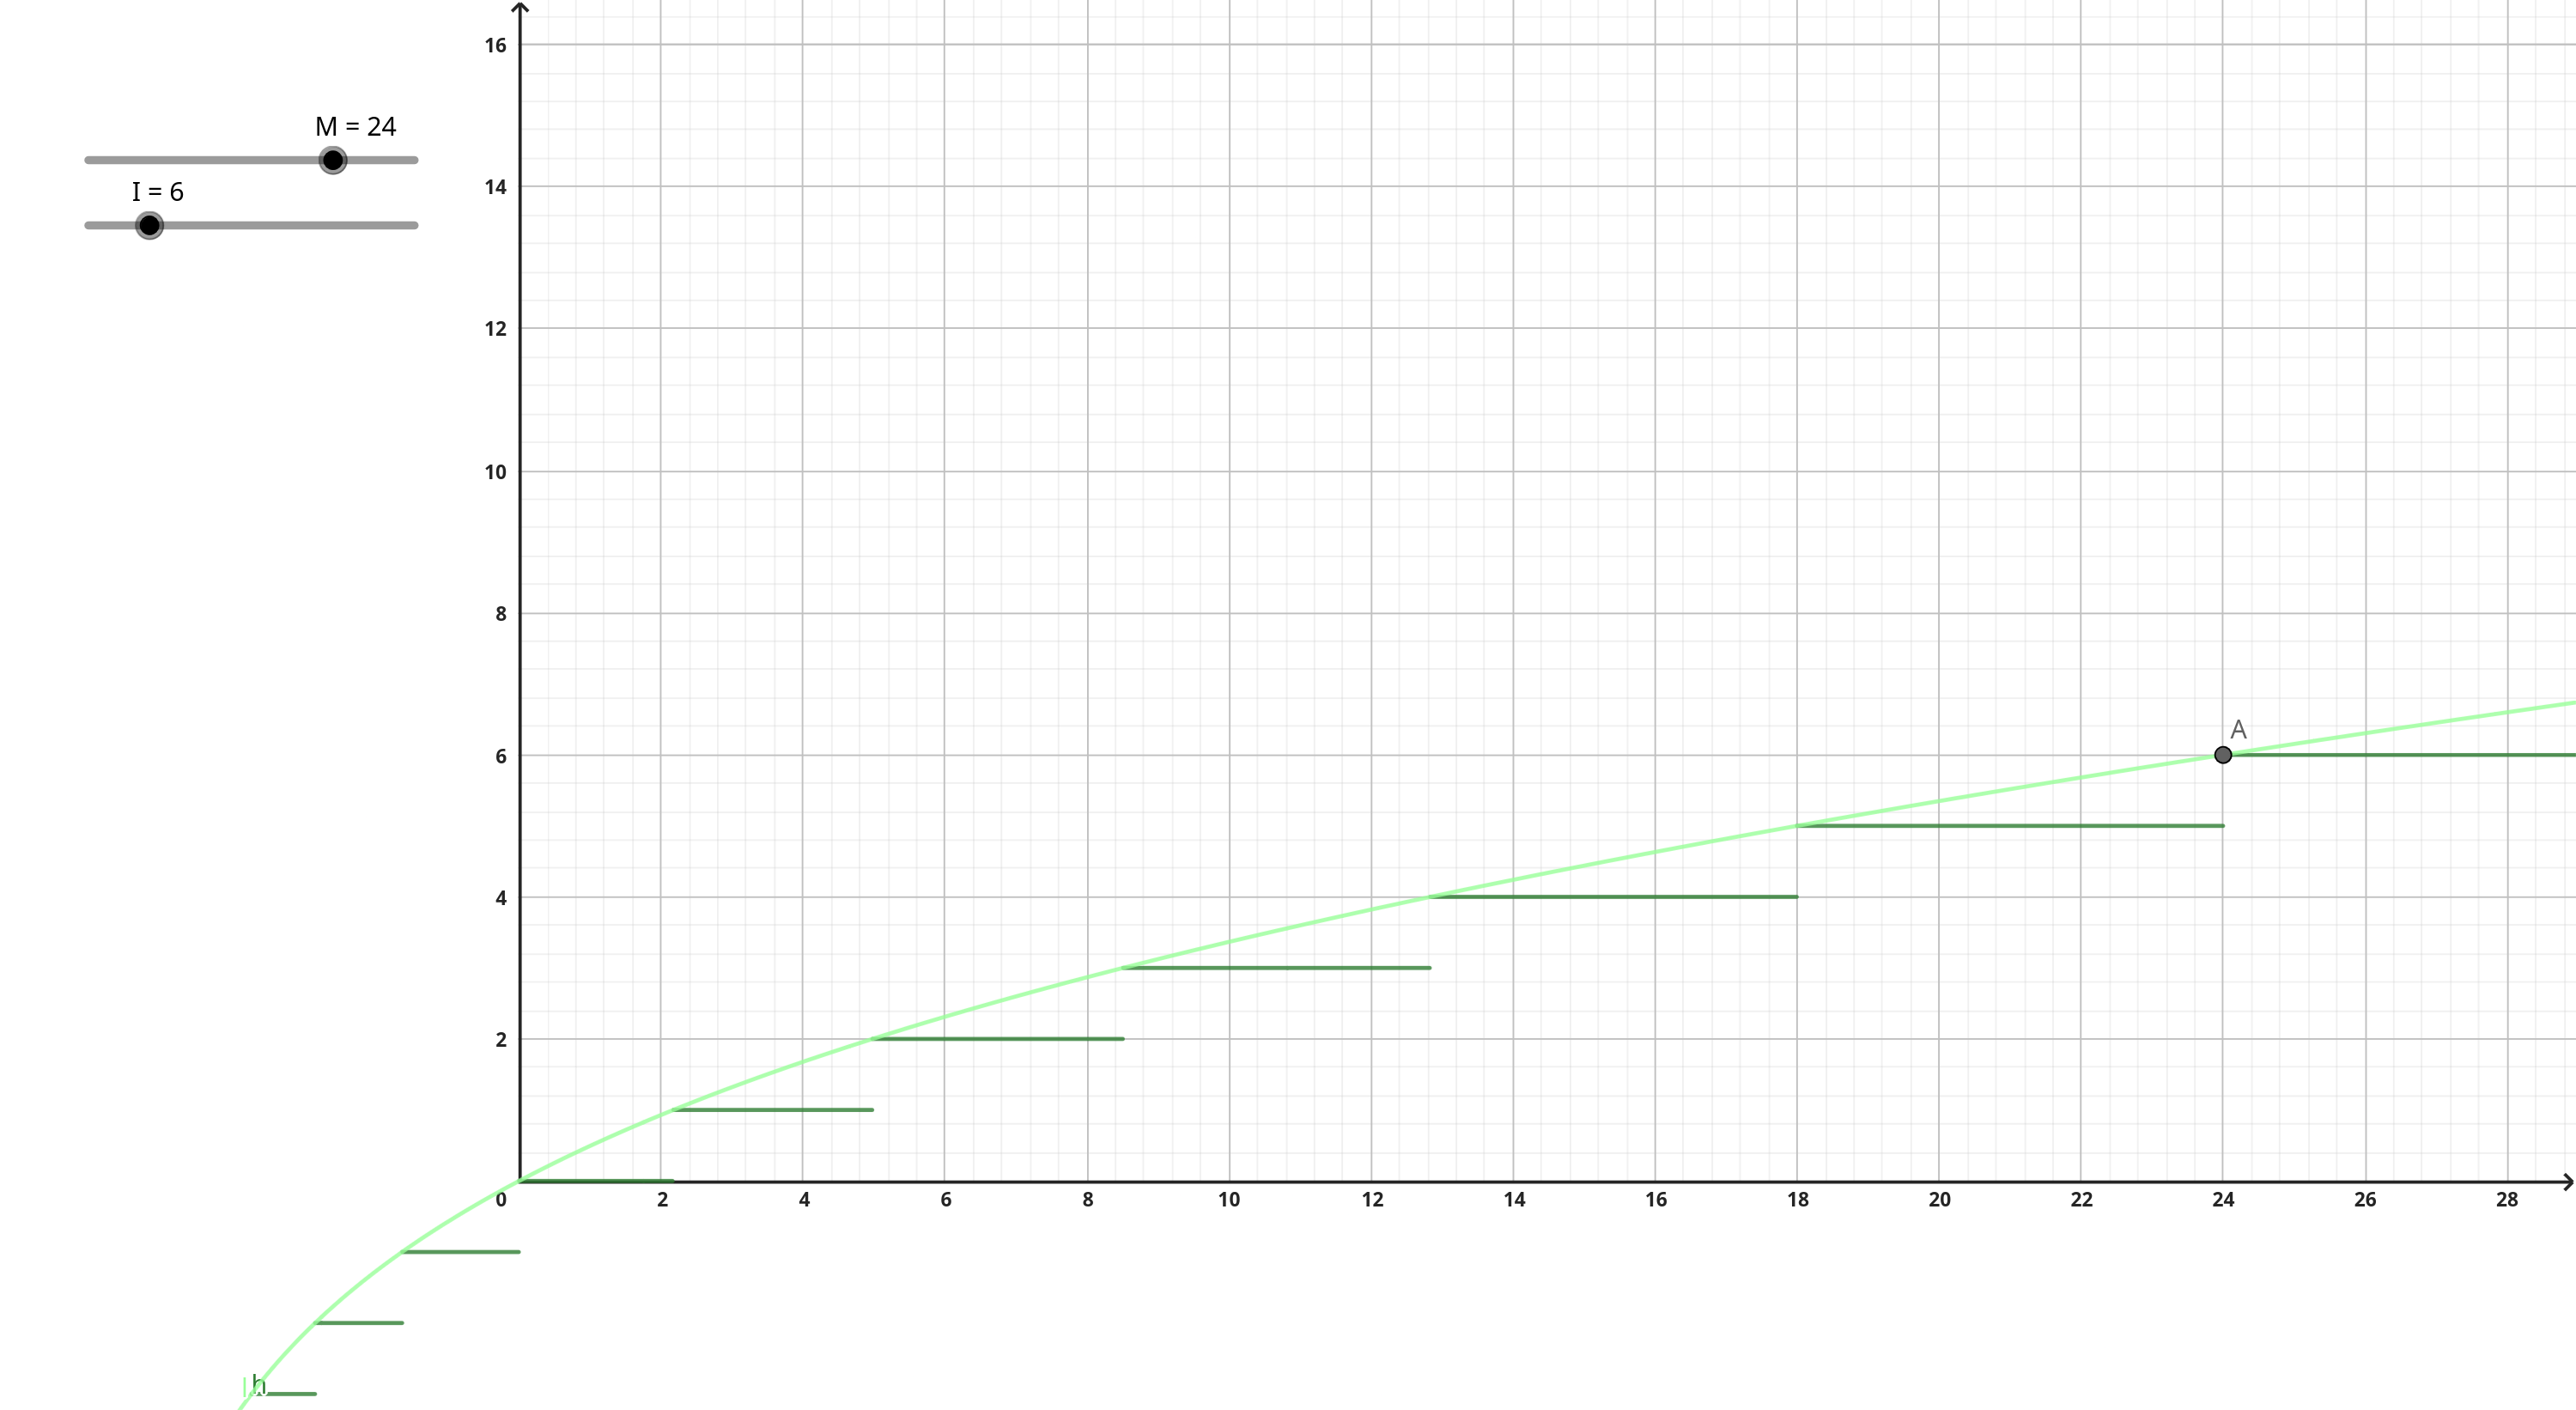
\includegraphics[width=0.78\textwidth]{imagenes/log_linear_blend_1.png}
    \caption{Ejemplo de la mezcla logarítmica-lineal utilizada por \texttt{Encoder}. La curva se interpreta como una transformación de la espera acumulada, no como una trayectoria de entrenamiento.}
    \label{fig:mezcla_log_lineal}
\end{figure}

\subsection{Espacio de Acciones y Enmascaramiento Dinámico}
\label{subsec:acciones_masking}

El espacio de acciones $\mathcal{A}_i = \{0, 1, \dots, K_i - 1\}$ representa el conjunto de fases verdes seleccionables por la intersección $i$. Los valores $m_i$ y $K_i$ difieren entre intersecciones según la geometría del cruce y las restricciones de maniobra, y cada agente dispone de un módulo de política propio sin compartición de parámetros; en ese sentido el conjunto de agentes es heterogéneo y la evaluación de \acrshort{acr-happo} se realiza sobre los espacios de observación y acción efectivos de cada escenario. En cruces con geometrías asimétricas o restricciones de maniobra, el entorno construye el conjunto de acciones admisibles y la capa personalizada \texttt{ActionMaskingTorchRLModule} aplica un enmascaramiento dinámico sobre los \glspl{logit} $z_i(a)$ antes del cómputo de la distribución \gls{softmax}. Los \glspl{logit} son puntuaciones reales sin normalizar producidas por la red; la función \gls{softmax} las transforma en probabilidades cuya suma es uno:
    \begin{equation}
\widetilde z_i(a,t) = z_i(a) + \log m_i(a,t), \qquad m_i(a,t) = \begin{cases}
    1 & \text{si } a \in \mathcal{A}^{\mathrm{adm}}_i(t) \\
    0 & \text{si } a \notin \mathcal{A}^{\mathrm{adm}}_i(t)
    \end{cases}
    \label{eq:action_mask}
    \end{equation}
donde $\mathcal{A}^{\mathrm{adm}}_i(t)\subseteq\mathcal{A}_i$ es el conjunto de acciones admisibles en el instante $t$, $m_i(a,t)$ es la máscara binaria correspondiente y $z_i(a)$ es la puntuación producida por la política. El entorno define $\mathcal{A}^{\mathrm{adm}}_i(t)=\{a_i^{\mathrm{actual}}\}$ durante una transición amarilla o mientras el tiempo de la fase corriente sea menor que $\max(t_{\min},t_{\mathrm{yellow}})$. Una vez satisfecha esa condición, quedan habilitadas las fases compatibles con la configuración del cruce. El término $\log m_i(a,t)$ vale $0$ para acciones admisibles y se limita a un entero negativo de magnitud máxima en aritmética de precisión finita para las inadmisibles, de modo que su contribución es despreciable tras la normalización. En IPPO, MAPPO y HAPPO la suma se aplica a los \textit{logits}; en IDQN se aplica a los valores $Q$ y también a la acción siguiente utilizada para el objetivo temporal, tanto en la red principal como en la red objetivo. La máscara evita acciones incompatibles, pero no reemplaza la lógica de transición amarilla del entorno, que se ejecuta después de aceptar un cambio de fase.

\subsection{Función de Recompensa Compuesta y Coordinación Vecinal}
\label{subsec:recompensa_coordinacion}

La función de recompensa representa el compromiso entre el desempeño operacional local y la cooperación distribuida. El código permite evaluar varias señales de tránsito; la selección de una señal no se interpreta como una superioridad universal, sino como una decisión experimental que se mantiene fija al comparar algoritmos dentro de un escenario. La tabla \ref{tab:alternativas_recompensa} resume las alternativas implementadas.

\begin{table}[H]
\centering
\caption{Señales de recompensa disponibles en el entorno.}
\label{tab:alternativas_recompensa}
\small
\begin{tabular}{p{4.0cm}p{7.2cm}p{3.0cm}}
\hline
\textbf{Identificador} & \textbf{Señal utilizada} & \textbf{Unidad o interpretación} \\
\hline
\texttt{diff\_halted} & Variación del número de vehículos detenidos entre pasos. & vehículos \\
\texttt{diff\_waitingTime} & Variación de la espera del último paso. & s \\
\shortstack[l]{\texttt{diff\_cumulative}\\\texttt{WaitingTime}} & Variación de la espera acumulada en los carriles de entrada. & vehículo$\cdot$s \\
\shortstack[l]{\texttt{negative\_waiting}\\\texttt{Time}\\\texttt{negative\_cumulative}\\\texttt{WaitingTime}} & Penalización directa de la espera instantánea o acumulada. & s o vehículo$\cdot$s \\
\shortstack[l]{\texttt{diff\_cumulative}\\\texttt{WaitingTime}\\\texttt{\_normalized}} & Variación acumulada dividida por la cantidad de vehículos considerada. & s \\
\texttt{pressure} & Negativo de la diferencia absoluta entre vehículos detenidos en entradas y salidas. & vehículos \\
\shortstack[l]{\texttt{negative\_queue}\\\texttt{\_length}} & Negativo de la cantidad de vehículos detenidos en los carriles de entrada. & vehículos \\
\hline
\end{tabular}
\end{table}

La tabla documenta las señales implementadas en el entorno; la disponibilidad de una clase no implica que haya sido comparada experimentalmente. En las campañas de ajuste de este capítulo se fija \texttt{reward\_key} = \path{diff_cumulative_waiting_time_with_neighbors}. Esta clave combina la señal diferencial de espera acumulada con una media sobre los vecinos mediante \texttt{NeighborhoodRelevanceReward}. En las líneas de base independientes (\acrshort{acr-ippo} e \acrshort{acr-idqn}), se fija de forma estricta $\rho_{\mathrm{coop}} = 0$, reduciendo la señal a la recompensa puramente local $R_i^{(t)} = L_i^{(t)}$. Para los métodos cooperativos (\acrshort{acr-mappo} y \acrshort{acr-happo}), el parámetro $\rho_{\mathrm{coop}} \in [0.0, 0.95]$ se optimiza mediante búsqueda bayesiana para determinar el grado óptimo de ponderación vecinal en cada escenario y arquitectura; una vez seleccionada la receta, su valor permanece fijo durante la confirmación y la evaluación reservada. No se agregan términos heurísticos adicionales. Las demás filas de la tabla se presentan como alternativas implementadas, no como funciones evaluadas, porque no existe para ellas una ejecución identificable por escenario, semilla, configuración y métrica.

\begin{enumerate}
    \item \textbf{Recompensa local diferencial ($L_i$):} cuantifica la variación del tiempo de espera acumulado entre pasos consecutivos. En esta sección, $W_{\text{acc},i}(t)$ representa la suma de los tiempos de espera de los vehículos presentes en los carriles de entrada controlados por la intersección $i$ en el paso $t$, expresada en vehículo$\cdot$segundo. La implementación activa selecciona esta señal mediante la opción de configuración \texttt{reward\_key} = \texttt{diff\_}\allowbreak\texttt{cumulative\_}\allowbreak\texttt{waiting\_}\allowbreak\texttt{time\_}\allowbreak\texttt{with\_}\allowbreak\texttt{neighbors}; su componente local utiliza esta diferencia sin dividirla por el número de vehículos. La ecuación \eqref{eq:recompensa_local} asigna una señal positiva cuando la espera disminuye:
    \begin{equation}
        L_i^{(t)} = W_{\text{acc}, i}(t-1) - W_{\text{acc}, i}(t)
        \label{eq:recompensa_local}
    \end{equation}
    \item \textbf{Señal vecinal ($N_i$):} corresponde al promedio de las señales locales obtenidas por las intersecciones del vecindario topológico directo $\mathcal{N}(i)$. Esta construcción incorpora al retorno del agente la evolución de los cruces inmediatamente conectados, pero no equivale a observar sus estados ni a optimizar una recompensa global. La ecuación \eqref{eq:recompensa_vecinal} supone $|\mathcal{N}(i)|>0$:
    \begin{equation}
        N_i^{(t)} = \frac{1}{|\mathcal{N}(i)|} \sum_{j \in \mathcal{N}(i)} L_j^{(t)}
        \label{eq:recompensa_vecinal}
    \end{equation}
    \item \textbf{Mezcla convexa:} se adopta una combinación convexa gobernada por el hiperparámetro $\rho_{\mathrm{coop}} \in [0, 0.95]$ para ponderar el componente local y el vecinal. La ecuación \eqref{eq:recompensa_compuesta} conserva las unidades de $L_i$ y $N_i$:
    \begin{equation}
        R_i^{(t)} = (1 - \rho_{\mathrm{coop}}) L_i^{(t)} + \rho_{\mathrm{coop}} N_i^{(t)} \quad \text{con} \quad \rho_{\mathrm{coop}} \in [0, 0.95]
        \label{eq:recompensa_compuesta}
    \end{equation}
    Si el vecindario es vacío, $|\mathcal{N}(i)|=0$, la implementación omite el promedio de la ecuación \eqref{eq:recompensa_vecinal} y define $R_i^{(t)}=L_i^{(t)}$. En \acrshort{acr-ippo} e \acrshort{acr-idqn}, $\rho_{\mathrm{coop}} = 0$ opera de forma fija como ancla puramente local descentralizada, garantizando que los agentes independientes no reciban retroalimentación de desempeño ajena. En \acrshort{acr-mappo} y \acrshort{acr-happo}, $\rho_{\mathrm{coop}} > 0$ modula la cooperación vecinal. En cada paso, el entorno forma el vector de recompensas $\mathbf{r}_t=(R_1^{(t)},\dots,R_N^{(t)})$ y entrega cada componente individual al módulo correspondiente; no se agregan sus componentes en una recompensa escalar global.
\end{enumerate}

\section{Implementación Algorítmica e Hiperparámetros}
\label{sec:implementacion_algoritmos}

Los cuatro algoritmos evaluados se integran en la \gls{acr-api} de Ray RLlib mediante el módulo de fábrica \texttt{algo\_factory.py}. \acrshort{acr-mappo} y \acrshort{acr-happo} utilizan \textit{learners} propios sobre PyTorch, mientras que \acrshort{acr-ippo} e \acrshort{acr-idqn} reutilizan las implementaciones de PPO y DQN de RLlib junto con módulos propios para el enmascaramiento de acciones.

\subsection{Mecanismos de Aprendizaje Independiente y Centralizado}
\label{subsec:mecanismos_algoritmos}

\begin{itemize}
    \item \textbf{\acrshort{acr-idqn} e \acrshort{acr-ippo} (Aprendizaje Independiente):} Cada intersección aprende una política local $\pi_{\theta_i}(a_i | o_i)$ tratando a los demás controladores como parte del entorno no estacionario. En \acrshort{acr-ippo}, cada agente cuenta con su propia red de valor local $V_{\phi_i}(o_i)$.
    \item \textbf{\acrshort{acr-mappo} (\acrshort{acr-ppo} Multi-Agente Centralizado \cite{yu2022surprising}):} Emplea el paradigma \acrshort{acr-ctde}. Durante la ejecución, cada actor selecciona acciones de forma descentralizada a partir de su observación local $o_i$. Durante el entrenamiento, el módulo \texttt{SharedCriticTorchRLModule} actúa como un crítico centralizado compartido multi-salida: recibe el vector de observaciones locales concatenadas $s = (o_1, o_2, \dots, o_N)$, que aporta contexto conjunto al crítico sin equivaler al estado Markoviano completo de la simulación, y produce $\mathbf{V}_{\phi}(s)=(V_{\phi,1}(s),\dots,V_{\phi,N}(s))$. Las recompensas, valores, objetivos y ventajas de \acrshort{acr-gae} ($\lambda_{\text{GAE}}$) se calculan por agente.
    \item \textbf{\acrshort{acr-happo} (\acrshort{acr-ppo} para Agentes Heterogéneos \cite{kuba2021trust}):} Su marco teórico canónico se apoya en el \textbf{Lema de Descomposición de Ventajas Multiagente}, cuya formulación utiliza una ventaja conjunta. La implementación de este trabajo constituye una adaptación: no aplica directamente ese lema, sino que inicializa los factores de actualización con ventajas individuales estandarizadas obtenidas mediante \acrshort{acr-gae} y los repondera secuencialmente. El crítico centralizado proporciona estimaciones de valor durante el entrenamiento, mientras que la reponderación secuencial descrita corresponde a la actualización de los actores; no se atribuye a esta secuencia una actualización secuencial del crítico. En cada \textit{epoch} de entrenamiento, los agentes se actualizan secuencialmente, sobre el lote completo y según un orden $(i_1, i_2, \ldots, i_N)$ re-sorteado, donde $N$ es el número total de agentes y $i_m$ es el agente ubicado en la posición $m$ de ese orden; cada actor recibe un único paso de gradiente por \textit{epoch}. Si $\overline{|A|}_i$ denota la media del valor absoluto de la ventaja individual ya estandarizada del agente $i$ en la muestra ---el conector de entrenamiento normaliza las ventajas por módulo antes de la actualización---, el hiperparámetro $p_{\text{greedy}}$ determina cómo se construye el orden: $0.0$ produce un orden aleatorio; $1.0$, un orden codicioso según $\overline{|A|}_i$; y un valor en $(0,1)$, un orden semi-codicioso que combina ambos criterios. Sea $\pi_{b}^{(i_m)}$ la política que recolectó la muestra y $\pi_{+}^{(i_m)}$ el actor de $i_m$ después de su actualización dentro del \textit{epoch} corriente. Para una observación $o$ y una acción $a$ de la muestra, la razón que se propaga a los agentes restantes es:
    \begin{equation}
        \rho_{\text{post}}^{(i_m)} = \frac{\pi_{+}^{(i_m)}(a|o)}{\pi_{b}^{(i_m)}(a|o)}
        \label{eq:happo_ratio_post_metodologia}
    \end{equation}
    La ecuación \eqref{eq:happo_ratio_post_metodologia} compara la política posterior a la actualización con la política de comportamiento que generó la muestra, el mismo denominador que utiliza el objetivo tipo \acrshort{acr-ppo} de la actualización. Para cada agente aún no actualizado $i_j$, con $j>m$, $M^{(i_j)}$ es el factor de ventaja reponderada del \textit{epoch} corriente, inicializado con su ventaja individual estandarizada al comienzo de ese \textit{epoch}. El factor se actualiza como
    \begin{equation}
        M^{(i_j)} \leftarrow M^{(i_j)} \cdot \rho_{\text{post}}^{(i_m)}, \qquad j>m.
        \label{eq:happo_factor_acumulado_metodologia}
    \end{equation}
    La ecuación \eqref{eq:happo_factor_acumulado_metodologia} incorpora al factor la razón de cada actor ya optimizado: la actualización de $i_1$ afecta a todos los agentes restantes del \textit{epoch}, la de $i_2$ a los que siguen en el orden, y así sucesivamente. Puesto que $M$ se reinicializa en cada \textit{epoch}, la propagación cubre únicamente a los agentes previos en el orden de ese \textit{epoch}, y no la secuencia completa de actualizaciones acumuladas desde la recolección.

    El procedimiento canónico de \acrshort{acr-happo} agrupa, en cambio, los pases internos de cada actor bajo un único factor secuencial; la diferencia se mantiene explícita porque afecta a la interpretación de las garantías: la mejora monótona corresponde al procedimiento teórico de región de confianza bajo sus supuestos explícitos y no se transfiere a esta variante con recorte. En la implementación evaluada, el coeficiente de la penalización de \acrshort{acr-kl} permanece fijo durante la actualización de \acrshort{acr-happo}.
\end{itemize}

La reponderación secuencial de ventajas individuales ofrece una forma de considerar políticas propias de intersecciones con acciones y condiciones de operación distintas, sin garantizar por sí misma un mejor control que MAPPO.

En los cuatro algoritmos, el entrenamiento consume observaciones del tránsito, fases ejecutadas, recompensas y observaciones siguientes para ajustar los parámetros de las redes. \acrshort{acr-idqn} conserva transiciones anteriores en un \textit{replay buffer} de episodios priorizado y multiagente; las variantes de \acrshort{acr-ppo} recolectan un \textit{rollout} con la política vigente y lo reutilizan durante una cantidad acotada de \textit{epochs}. Cada \textit{epoch} recorre el conjunto recolectado; en \acrshort{acr-ippo} y \acrshort{acr-mappo} el lote se subdivide en \textit{minibatches} y cada uno produce una actualización, mientras que en \acrshort{acr-happo} el lote no se subdivide y cada actor realiza un único paso de gradiente completo por \textit{epoch}. El optimizador, los búferes y los críticos pertenecen al proceso de aprendizaje: durante la ejecución del control, cada intersección solo necesita su observación local y la red entrenada que asigna valores o probabilidades a las fases admisibles. Por tanto, la salida del entrenamiento es una política parametrizada, no un plan semafórico fijo.

\section[Búsqueda de Hiperparámetros (HPO)]{Búsqueda de Hiperparámetros (\acrshort{acr-hpo})}
\label{sec:experimentos_hiperparametros}

La búsqueda de hiperparámetros se ejecutó con Optuna \cite{akiba2019optuna}, Ray Tune y el algoritmo de poda asíncrona \gls{acr-asha} \cite{li2020system} para las combinaciones sintéticas de algoritmo, escenario y arquitectura. La Ciudad de Mendoza se definió como un estudio separado, cuya búsqueda se inicia después del cierre de los estudios y la confirmación sintéticos. La receta sintética no se transfiere automáticamente: sus resultados pueden utilizarse, a lo sumo, para acotar el espacio de exploración de Mendoza.

Antes del muestreo se fijaron los parámetros que definen la semántica de la interacción. En particular, $\gamma=0,99$ se mantuvo constante en MAPPO, HAPPO, IPPO e IDQN como decisión de diseño informada por las configuraciones de referencia del proyecto, y no como un óptimo universal. También se fijaron la métrica de carril, la señal de recompensa y el calibrado $M_{\mathrm{lane}}$ por escenario. Las arquitecturas \texttt{h128} y \texttt{h256} no se mezclan dentro de un mismo estudio: cada una recibe un estudio independiente y se comparan después mediante métricas físicas. La métrica de carril, la recompensa, $M_{\mathrm{lane}}$ y el modo de interacción se mantienen fijos por escenario. En cambio, el número de intervalos del codificador es un hiperparámetro: modifica la resolución con que se representa cada carril y, por ello, se explora explícitamente junto con los parámetros de aprendizaje.

\begin{enumerate}
    \item \textbf{Etapa 1 (exploración bayesiana amplia):} muestreo mediante \gls{acr-tpe}. El presupuesto nominal es de 100 pruebas por combinación; el valor de 150 corresponde al límite máximo previsto para una eventual ampliación y no a una segunda etapa de búsqueda. ASHA aplica poda temprana con período de gracia de 10 iteraciones y factor de reducción 4; las pruebas podadas no integran el conjunto de candidatos finales. Se evalúan las arquitecturas compacta (\texttt{h128}: $[128, 128]$) y ancha (\texttt{h256}: $[256, 256]$) como estudios independientes de Ray Tune. El espacio registrado comprende 13 dimensiones para \acrshort{acr-mappo} y 13 parámetros nominales para \acrshort{acr-ippo}, de los cuales 12 son efectivos porque $\rho_{\mathrm{coop}}=0$ se fija. Para \acrshort{acr-happo} se registran 14 parámetros, aunque dos no modifican la actualización y el espacio efectivo comprende 12 dimensiones:
    \begin{itemize}
        \item $\rho_{\mathrm{coop}} \in [0.0, 0.95]$ (solo \acrshort{acr-mappo} y \acrshort{acr-happo}, \texttt{uniform})
        \item $\alpha_{\mathrm{lr}} \in [3\times 10^{-5}, 10^{-3}]$ (\texttt{loguniform})
        \item $\epsilon_{\mathrm{clip}} \in [0.10, 0.22]$ (\texttt{uniform})
        \item $\lambda_{\text{GAE}} \in [0.88, 0.99]$ (\texttt{uniform})
        \item $c_{\text{entropy}} \in [0.0, 0.01]$ (\texttt{uniform})
        \item $\text{grad\_clip} \in [0.25, 5.0]$ (\texttt{loguniform})
        \item $c_{\text{KL}} \in [0.05, 0.5]$ (\texttt{loguniform})
        \item $d_{\text{KL\_target}} \in [0.005, 0.03]$ (\texttt{loguniform})
        \item $\text{vf\_clip} \in [5.0, 20.0]$ (\texttt{loguniform})
        \item $K \in [5, 15]$ para \acrshort{acr-mappo} e \acrshort{acr-ippo}, y $K \in [5, 18]$ para \acrshort{acr-happo} (\texttt{randint})
        \item $N_{\text{episodes}} \in [2, 12]$ (\texttt{randint})
        \item $I \in [4, 64]$ (\texttt{randint})
        \item $B_{\text{mini}} \in \{128, 256, 512\}$ (\texttt{choice})
        \item $p_{\text{greedy}} \in [0.20, 0.90]$ (solo \acrshort{acr-happo}, \texttt{uniform})
    \end{itemize}
    Parámetros fijos: $\texttt{lane\_metric}=\texttt{acc\_waiting\_time}$, $\text{use\_kl\_loss} = \text{True}$, $\gamma=0,99$ y, para \acrshort{acr-ippo}, $\rho_{\mathrm{coop}}=0$ fijo. Para \acrshort{acr-idqn}, el espacio específico de diez dimensiones reemplaza los parámetros de \acrshort{acr-ppo} por tasa de aprendizaje $[10^{-5},10^{-3}]$, lotes $\{64,128,256,512\}$, \texttt{grad\_clip} $\in\{0,5;1;2;5;10\}$, actualización de la red objetivo $\{500,1000,2000,5000\}$ pasos, decaimiento de $\varepsilon$ en $\{5000,10000,20000\}$ pasos, $\varepsilon_{\mathrm{final}}\in[0,02,0,10]$, retorno de $n$ pasos $\{1,3,5\}$ y comienzo del aprendizaje $\{1000,2000,5000\}$ pasos, también con recompensa estrictamente local ($R_i = L_i$). En todos los algoritmos se explora $I\in[4,64]$ mediante \texttt{tune.randint(4,65)}, cuyo extremo superior no se incluye, y se fija el valor de saturación $M_{\mathrm{lane}}$ calibrado para cada escenario. En \acrshort{acr-happo}, las dimensiones asociadas al \textit{minibatch} y al objetivo de \acrshort{acr-kl} se muestrean y registran, pero no modifican su actualización, que opera con lote completo por actor y coeficiente de \acrshort{acr-kl} fijo; la búsqueda efectiva sobre \acrshort{acr-happo} comprende doce dimensiones. En los escenarios sintéticos, las semillas de entrenamiento de HPO son $\{101,137,179\}$ para $3\times1$, $3\times3$ y $4\times4\_H$, respectivamente, y las de evaluación son $\{100101,100137,100179\}$. La búsqueda en cada escenario sintético dispuso de una única semilla de entrenamiento, de modo que el ordenamiento de candidatos queda expuesto a esa realización pseudoaleatoria; la confirmación sobre diez semillas se definió para controlar ese riesgo de selección. Para Mendoza, el presupuesto y los conjuntos de semillas deben fijarse antes de iniciar su campaña y mantenerse separados de los utilizados en la evaluación reservada.
    \item \textbf{Etapa 2 (confirmación pareada):} se previó un reentrenamiento a presupuesto completo sobre las semillas de confirmación definidas por escenario. En MAPPO y HAPPO, el diseño contrasta el $\rho_{\mathrm{coop}}$ seleccionado con la línea base puramente local ($\rho_{\mathrm{coop}} = 0$). IPPO e IDQN se mantienen como líneas de base de aprendizaje independiente con recompensa puramente local, con sus propias recetas seleccionadas y las mismas reglas de evaluación reservada. Para Mendoza se definió una secuencia propia de ajuste, congelamiento y confirmación, posterior al cierre sintético. Dado que el tamaño del lote de aprendizaje forma parte del espacio de ajuste, las cuarenta iteraciones fijan el número de actualizaciones y no la experiencia total consumida; por ello, cada ejecución registra los pasos de entorno muestreados de forma acumulada (\texttt{num\_env\_steps\_sampled}) para informar, junto con el desempeño, la experiencia requerida para alcanzarlo. Las comparaciones entre familias se formulan sobre las políticas finales evaluadas bajo el mismo horizonte, la misma demanda y las mismas semillas, y no como afirmaciones de eficiencia muestral entre algoritmos.
\end{enumerate}

La selección de candidatos minimiza la métrica física \texttt{metric\_objective}, que en la campaña corresponde a la espera media estable por vehículo insertado. Sea $w_r$ la espera media de los vehículos insertados en la iteración de entrenamiento $r$. Para diagnosticar inestabilidad se calcula el incremento positivo
\begin{equation}
    X_r = \max\{0, w_r-w_{r-1}\}.
    \label{eq:incremento_espera_iteracion}
\end{equation}
La colección de realizaciones $\{X_r\}$ corresponde a \texttt{positive\_interiteration\_increases}. Para la fracción superior $\alpha_{\mathrm{CVaR}}=0,2$ se utiliza el estimador empírico de cola:
\begin{equation}
    \widehat{\operatorname{CVaR}}_{\alpha_{\mathrm{CVaR}}}(X) = \frac{1}{k}\sum_{j=1}^{k}X_{(j)}, \qquad k=\max\{1,\lceil m\alpha_{\mathrm{CVaR}}\rceil\},
    \label{eq:cvar_incrementos_espera}
\end{equation}
La ecuación \eqref{eq:cvar_incrementos_espera} reproduce el cálculo implementado: $m$ es la cantidad de incrementos finitos disponibles, $X_{(j)}$ son esos incrementos ordenados de mayor a menor y $k$ garantiza que siempre se utilice al menos una observación. Por tanto, la penalización es un promedio empírico del $20\%$ superior, no una garantía de ausencia de \textit{gridlock}. La espera $w_r$ se obtiene de \texttt{TripInfo} y se expresa en segundos por vehículo insertado.
\begin{equation}
    \text{metric\_objective}_r = w_r + 1,0 \cdot \widehat{\operatorname{CVaR}}_{0,2}(X)
    \label{eq:objetivo_estable_espera}
\end{equation}
La ecuación \eqref{eq:objetivo_estable_espera} se informa sobre las últimas 10 iteraciones, después de excluir las primeras 5 del historial de estabilidad. La primera parte prioriza una espera media baja y el segundo término penaliza aumentos recientes; el coeficiente $1,0$ es adimensional. Los candidatos se ordenan de menor a mayor por \texttt{metric\_objective}; cuando existe una métrica de evaluación válida, la espera media de evaluación se utiliza como segunda clave y, si no existe, se utiliza la espera media de entrenamiento. La ejecución debe alcanzar las 40 iteraciones y aportar métricas derivadas de \texttt{TripInfo} aptas para el ordenamiento. La completitud, la inserción, los teletransportes y la pérdida temporal se conservan para la confirmación.

\subsection{Selección y congelamiento de las configuraciones finales}
\label{subsec:seleccion_configuraciones_finales}

La selección se realiza por separado para cada combinación de algoritmo, escenario y arquitectura. Primero se consideran elegibles las pruebas que alcanzan las 40 iteraciones y aportan las métricas requeridas, derivadas de \texttt{TripInfo}: el selector exige que la métrica primaria y la secundaria estén presentes, sean convertibles a número y no sean \texttt{NaN}. La finitud de las magnitudes físicas se garantiza aguas arriba, en la extracción de métricas: el lector de \texttt{TripInfo} aborta ante atributos infinitos o negativos, valores no numéricos e identificadores de vehículo duplicados, de modo que una ejecución con telemetría inválida no produce métrica elegible.

El selector ordena a continuación por \texttt{metric\_objective} en sentido ascendente. Cuando está disponible, \texttt{tripinfo/}\allowbreak\texttt{eval\_}\allowbreak\texttt{mean\_}\allowbreak\texttt{waiting\_}\allowbreak\texttt{time\_}\allowbreak\texttt{inserted} constituye la segunda clave; en su ausencia se utiliza \texttt{tripinfo/}\allowbreak\texttt{mean\_}\allowbreak\texttt{waiting\_}\allowbreak\texttt{time\_}\allowbreak\texttt{inserted}. Esta regla mantiene un ordenamiento reproducible, aunque la segunda clave puede provenir de evaluación o de entrenamiento; esa circunstancia se registra en el manifiesto de cada receta.

Las arquitecturas \texttt{h128} y \texttt{h256} se exploran en estudios independientes y se comparan después mediante las mismas métricas físicas. La receta final conserva el identificador del estudio y del ensayo seleccionado, junto con la referencia al checkpoint generado al cierre del reentrenamiento, lo que asegura la trazabilidad de la configuración y de la política evaluada.

La receta congelada conserva todos los parámetros que determinan la interacción —\texttt{reward\_key}, \texttt{lane\_metric}, $M_{\mathrm{lane}}$ y $\gamma$— junto con los hiperparámetros de optimización seleccionados. No se modifican al evaluar las semillas reservadas del escenario correspondiente. Para Mendoza se definió una selección de recetas propia para MAPPO, HAPPO, IPPO e IDQN, sin transferencia automática desde las redes sintéticas; la limitación del aforo se trata como una restricción de validez externa y no como una razón para excluir el ajuste del controlador. La política de cada evaluación reservada proviene del reentrenamiento de la receta congelada y sus métricas no alimentan ninguna nueva decisión de ajuste.

\subsection{Infraestructura de Cómputo y Orquestación}
\label{subsec:infraestructura_hpc}

Dado el tamaño del espacio de búsqueda y el costo computacional de la simulación microscópica en \acrshort{acr-sumo}, la exploración y el entrenamiento final se desplegaron en los clústeres de cómputo \textbf{Toko} (\gls{acr-ccar} - \gls{acr-fcefn} / UNCuyo / \gls{acr-conicet}) y \textbf{Mendieta} (\gls{acr-ccad} - Universidad Nacional de Córdoba).

La ejecución distribuida se gestionó mediante el sistema de colas \acrshort{acr-slurm}. Se aplicaron las siguientes medidas:
\begin{itemize}
    \item \textbf{Aislamiento de procesos Ray en un nodo:} configuración de instancias Ray de nodo único (\texttt{setup\_ray\_single\_node}) con asignación dinámica de puertos basada en el identificador de trabajo:
    \begin{equation}
        \text{ray\_port} = 20000 + (\text{SLURM\_JOB\_ID} \pmod{20000})
        \label{eq:puerto_ray}
    \end{equation}
    La ecuación \eqref{eq:puerto_ray} transforma el identificador del trabajo en un puerto dentro de un intervalo acotado. En ella, \texttt{SLURM\_JOB\_ID} es el identificador entero del trabajo y $\pmod{20000}$ devuelve su resto al dividirlo por $20.000$. Por tanto, el puerto calculado pertenece al intervalo entero $[20000,39999]$; la fórmula reduce la probabilidad de colisión entre trabajos concurrentes, pero no constituye una reserva de puertos del sistema. Se utiliza junto con la autodetección de dirección IP mediante \texttt{hostname --ip-address}.
    \item \textbf{Gestión de E/S en almacenamiento local} (\texttt{/scratch}): para evitar saturar el sistema de archivos distribuido en red (\gls{acr-nfs}) con la telemetría microscópica de \acrshort{acr-sumo} (\texttt{tripinfo.xml}, \texttt{summary.xml}), las simulaciones y la recolección de trayectorias se ejecutaron en el almacenamiento local de cada nodo (\texttt{/scratch/\$USER/ray\_tmp/}).
    \item \textbf{Persistencia ante preempción:} los scripts de envío incorporan trampas de señales \acrshort{acr-posix} (\texttt{trap ... EXIT USR1 TERM INT}).\\
    Estas trampas sincronizan mediante \texttt{rsync} los resultados y las bases de datos SQLite de Optuna con el almacenamiento persistente del usuario (\texttt{\$HOME}), en el directorio \path{ray\_results/}. Esto permite reanudar los trabajos mediante \texttt{Tuner.restore()}.
\end{itemize}

\section{Evaluación de Rendimiento}
\label{sec:experimentos_evaluacion}

La evaluación de los modelos con hiperparámetros congelados se definió por escenario y bajo tres niveles de comparación. Cada entrenamiento independiente produce una política asociada a una semilla de entrenamiento; sus episodios de evaluación se agregan primero dentro de esa ejecución. Luego se comparan las ejecuciones independientes, que constituyen la unidad experimental.

Para los escenarios sintéticos se definieron las semillas de confirmación de entrenamiento $\{211,223,227,229,233,239,241,251,257,263\}$ y sus semillas de evaluación correspondientes $\{200211,\ldots,200263\}$. La Ciudad de Mendoza se reservó como un estudio separado, con sus propias semillas y configuración de campaña, posteriores al cierre sintético. Cada receta se evalúa sin nuevas decisiones de ajuste con las semillas reservadas del escenario. Estas semillas son diferentes de las utilizadas para seleccionar candidatos y no se las denomina \acrshort{acr-ood}, porque la demanda y la topología permanecen dentro de la familia definida para cada escenario.

Las partidas de los cuatro escenarios provienen de flujos congelados en archivos de rutas, que \acrshort{acr-sumo} convierte en vehículos durante la ejecución: en Mendoza los instantes de inserción se sortean según el proceso exponencial descrito en la sección \ref{subsubsec:mendoza_demanda_dinamica}, y en las redes sintéticas los flujos siguen intervalos regulares por \texttt{vehsPerHour}. En ambos casos la semilla de \acrshort{acr-sumo} gobierna los componentes pseudoaleatorios del simulador ---asignación de tipos vehiculares, empates de ruteo y evolución microscópica--- además de las llegadas cuando estas son estocásticas. La semilla del generador de demanda de cada escenario queda registrada en su manifiesto.

La confirmación pareada de cooperación se definió para contrastar el valor seleccionado de $\rho_{\mathrm{coop}}$ con el ancla $\rho_{\mathrm{coop}}=0$ en MAPPO y HAPPO, que son las familias para las que se implementa este contraste. IPPO e IDQN se utilizan como líneas de base de aprendizaje independiente: sus recetas se seleccionan con el mismo criterio físico de HPO y sus políticas congeladas se evalúan bajo las mismas semillas reservadas para la comparación final. A diferencia de MAPPO y HAPPO, que incorporan la recompensa cooperativa local-vecinal ($\rho_{\mathrm{coop}} > 0$) y entrenamiento centralizado, IPPO e IDQN operan exclusivamente con la señal de recompensa local ($R_i = L_i$, fijando $\rho_{\mathrm{coop}} = 0$) para representar el paradigma descentralizado e independiente.

El análisis experimental evalúa la hipótesis de si \acrshort{acr-happo} logra superar a las líneas de base de aprendizaje multiagente (\acrshort{acr-mappo}, \acrshort{acr-ippo} e \acrshort{acr-idqn}) en escenarios con disparidad de fases y heterogeneidad de flujos. De forma complementaria, cada política aprendida se contrasta contra el controlador semafórico de tiempo fijo del mismo escenario, que actúa como ancla operacional no aprendida de referencia. Para una métrica $M$ cuyo valor menor es preferible, se informa la diferencia relativa
\begin{equation}
    \Delta_M = 100\,\frac{M_{\mathrm{politica}}-M_{\mathrm{fijo}}}{M_{\mathrm{fijo}}}.
    \label{eq:diferencia_relativa_controlador}
\end{equation}
Para tasas de inserción, completitud o finalización, cuyo valor mayor es preferible, se informa además el cambio porcentual con el signo interpretado según esa dirección. La ecuación \eqref{eq:diferencia_relativa_controlador} permite comparar redes con distinta cantidad de intersecciones sin confundir una reducción absoluta de segundos con una mejora relativa.

Las métricas se presentan en tablas por escenario y algoritmo, con media, mediana, desviación estándar e intervalo de confianza del 95\% por bootstrap percentil. La unidad de remuestreo es la ejecución completa asociada a una semilla, no cada vehículo individual ni cada episodio de una misma política. Para la confirmación pareada se utiliza el procedimiento \texttt{paired\_bootstrap}: calcula la diferencia candidato menos línea base dentro de cada semilla, realiza 20.000 remuestreos con semilla $910001$ y devuelve el intervalo percentil, la diferencia media, la diferencia relativa y la proporción de remuestreos cuya media de diferencias es favorable. Esta proporción no se interpreta como una probabilidad posterior de superioridad.

El remuestreo refleja la incertidumbre de las diez ejecuciones disponibles sin aumentar el tamaño muestral: la precisión de los intervalos descansa en esa muestra. Las métricas de conteo se informan también de forma absoluta para evitar que una razón inestable o un denominador pequeño oculte el comportamiento de la red.

Cada métrica se calcula sobre una población y una ventana declaradas. La espera media de vehículos insertados utiliza como denominador los registros cuyo instante de partida pertenece a la ventana controlada; los viajes inconclusos aportan la espera observada hasta el cierre, que no equivale a su tiempo total de viaje. Si el denominador de una tasa o diferencia relativa es cero, el cambio relativo se informa como no definido y se conserva la diferencia absoluta. Para las tasas de completitud, inserción y finalización se reportan también los puntos porcentuales de diferencia. Cuando todos los tiempos de espera intersección son cero, el Gini se informa como cero por definición operacional.

La tabla \ref{tab:metricas_evaluacion} fija qué magnitudes se consideran primarias, secundarias o de control.

\begin{table}[H]
\centering
\caption{Métricas utilizadas para presentar y controlar la evaluación final.}
\label{tab:metricas_evaluacion}
\small
\begin{tabular}{p{3.8cm}p{4.4cm}p{5.4cm}}
\hline
\textbf{Métrica} & \textbf{Papel} & \textbf{Justificación} \\
\hline
Espera media de vehículos insertados & Primaria & Resume la demora experimentada por la demanda que efectivamente ingresa en la ventana controlada; es el objetivo de HPO. \\
Pérdida temporal media (\texttt{timeLoss}) & Secundaria & Captura desaceleraciones y circulación por debajo de la velocidad ideal que no siempre se reflejan en detenciones completas. \\
CR, IR y CI & Eficiencia y atención de demanda & Distinguen una política que reduce la espera de una que simplemente impide insertar vehículos o deja viajes pendientes. La CI mide específicamente la fracción de vehículos insertados en la ventana que completa su itinerario en ella. \\
Teletransportes iniciados/finalizados & Control de estabilidad & Detecta bloqueos o colapsos que SUMO resuelve mediante su mecanismo de \textit{teleport}. \\
Media, desviación, máximo, rango y Gini de espera por intersección & Equidad espacial & Indican si la mejora media se obtiene sacrificando accesos secundarios o concentrando la demora en pocos nodos. \\
\hline
\end{tabular}
\end{table}

El objetivo de HPO se utiliza exclusivamente para ordenar configuraciones; la evaluación final no reemplaza la espera media por su término de estabilidad. Se reportan por separado la espera estable, la espera media sin penalización y el incremento CVaR. No se aplican umbrales de descarte definidos después de observar los resultados: cualquier reducción de completitud, aumento de teletransportes o deterioro de equidad se muestra como resultado de control y se discute junto con la métrica primaria. Así se evita convertir una decisión posterior en un criterio de selección encubierto.

En síntesis, el diseño experimental estima el cambio de la espera media por vehículo insertado contrastando prioritariamente a HAPPO frente a MAPPO, IPPO e IDQN, utilizando el control de tiempo fijo del mismo escenario como ancla operacional de referencia, con la ejecución completa de entrenamiento como unidad experimental y con CR, IR, CI, teletransportes y equidad espacial como controles de atención a la demanda y de estabilidad. Sus principales restricciones de validez externa son el carácter restringido por datos del escenario de la Ciudad de Mendoza y la línea base de tiempo fijo generada por \acrshort{acr-sumo} ---que no reconstruye los planes semafóricos municipales---. El capítulo \ref{capitulo:resultados} presenta los resultados obtenidos con este protocolo.
